\documentclass[a4paper,11pt]{article}
\usepackage[T1]{fontenc}
\usepackage[utf8]{inputenc}
\usepackage{lmodern}
\usepackage[francais]{babel}

% title info
\newcommand{\ititle}{Projet IA04 - NF28} % title
\newcommand{\isubtitle}{Colladia, éditeur de diagramme collaboratif}
\newcommand{\iauthor}{Jean Vintache\\Florian Impellettieri\\Charles Menier\\Marouane Hammi\\Adrien Jacquet} % author
\newcommand{\idate}{\today} % date

\usepackage{graphicx}
\usepackage{tabularx}
\usepackage{lastpage}
\usepackage[top=2.75cm, bottom=3cm, left=2cm, right=2cm]{geometry}
\usepackage[colorlinks=true, urlcolor=blue, linkcolor=black, citecolor=black]{hyperref}
\usepackage{calc}
\usepackage{amsmath} % equation align
\usepackage{amsfonts}
\usepackage{amssymb}
\usepackage{fancyhdr}
\usepackage[format=hang, width=.8\textwidth, labelfont=sc]{caption}
\usepackage[format=hang, width=.8\textwidth, labelfont=normalfont]{subcaption}
% \usepackage[labelformat=empty]{caption} % no label before caption
\usepackage{verbatim}

% paragraph and subparagraph as level 4 and 5 sections
\usepackage{titlesec}
\usepackage{titletoc}
\setcounter{secnumdepth}{5}
\setcounter{tocdepth}{5}
\titleformat{\paragraph} [hang] {\normalfont\normalsize\bfseries} {\theparagraph} {1em} {}
\titleformat{\subparagraph} [hang] {\normalfont\normalsize\bfseries} {\thesubparagraph} {1em} {}

% lists config
\usepackage{enumitem}
\setlist[itemize]{label=-}

% replace no-break space
\DeclareUnicodeCharacter{00A0}{ }

% header & footer
\pagestyle{fancy}
\fancyhf{}
\setlength{\headheight}{14pt}
\lhead{{\small \ititle}}
\rhead{{\small \isubtitle}}
\lfoot{}
\rfoot{\hrule\vspace{.1cm}\thepage /\pageref*{LastPage}}

\usepackage{color}
\usepackage{xcolor}
\usepackage{listings}

% define colors
\definecolor{kblue}{HTML}{204A87}
\definecolor{cred}{HTML}{A52A2A}
\definecolor{sorange}{HTML}{FF7800}
\definecolor{ngreen}{HTML}{4E9A06}
\definecolor{pprocess}{HTML}{339999}
\definecolor{opbrown}{HTML}{AB7A00}

% code highlight style
\lstdefinestyle{lstyle}{
	aboveskip=9mm,
	belowskip=1mm,
	basicstyle=\ttfamily\footnotesize,
	keywordstyle=\bfseries\color{kblue},
	commentstyle=\color{cred},
	stringstyle=\color{sorange},
	emphstyle=\color{pprocess},
	breaklines=true,
	tabsize=3,
	showstringspaces=false,
	captionpos=b
% 	literate={=}{{{\color{opbrown}=}}}1
}

% language
\lstset{
	language=Java,
	frame=single,
	numbers=left,
	numberstyle=\footnotesize,
	style=lstyle,
	emph={},
	morekeywords={None, False, True},
	extendedchars=true
}

% utf8 char
\lstset{literate=
  {á}{{\'a}}1 {é}{{\'e}}1 {í}{{\'i}}1 {ó}{{\'o}}1 {ú}{{\'u}}1
  {Á}{{\'A}}1 {É}{{\'E}}1 {Í}{{\'I}}1 {Ó}{{\'O}}1 {Ú}{{\'U}}1
  {à}{{\`a}}1 {è}{{\`e}}1 {ì}{{\`i}}1 {ò}{{\`o}}1 {ù}{{\`u}}1
  {À}{{\`A}}1 {È}{{\'E}}1 {Ì}{{\`I}}1 {Ò}{{\`O}}1 {Ù}{{\`U}}1
  {ä}{{\"a}}1 {ë}{{\"e}}1 {ï}{{\"i}}1 {ö}{{\"o}}1 {ü}{{\"u}}1
  {Ä}{{\"A}}1 {Ë}{{\"E}}1 {Ï}{{\"I}}1 {Ö}{{\"O}}1 {Ü}{{\"U}}1
  {â}{{\^a}}1 {ê}{{\^e}}1 {î}{{\^i}}1 {ô}{{\^o}}1 {û}{{\^u}}1
  {Â}{{\^A}}1 {Ê}{{\^E}}1 {Î}{{\^I}}1 {Ô}{{\^O}}1 {Û}{{\^U}}1
  {œ}{{\oe}}1 {Œ}{{\OE}}1 {æ}{{\ae}}1 {Æ}{{\AE}}1 {ß}{{\ss}}1
  {ç}{{\c c}}1 {Ç}{{\c C}}1 {ø}{{\o}}1 {å}{{\r a}}1 {Å}{{\r A}}1
  {€}{{\EUR}}1 {£}{{\pounds}}1
}

% use with \begin{lstlisting}[caption={#}, language=#] # \end{lstlisting}
% or \lstinline[caption={#}, language=#]$#$ --> $ can be replaced by any other character not used in the code


\begin{document}
% title
\newcommand*{\ClipSep}{0.4cm}
\begin{center}
	\hspace*{-1.8cm}
	\begin{tikzpicture}
		\node [inner sep=0pt] at (0,0) {
\includegraphics[width=\textwidth+3cm]{img/colladia-banner}};
		\draw [white, rounded corners=\ClipSep, line width=\ClipSep] 
				(current bounding box.north west) -- 
				(current bounding box.north east) --
				(current bounding box.south east) --
				(current bounding box.south west) -- cycle
				;
	\end{tikzpicture}~\\\vspace*{.5cm}
% 	\vspace*{.75cm}{\huge \textsc{\ititle}}~\\
% 	\vspace{.25cm}{\LARGE \isubtitle}~\\
	\vspace{1cm}{\large\iauthor}~\\
	\vspace{.6cm}{\large\idate}
\end{center}
\vspace*{-1.5cm}

% table of content (titlepage)
% \vspace{\fill}
% \tableofcontents

% logo
\vspace{\fill}
\hspace{-1.25cm}
\includegraphics[width=5cm]{img/utc-logo.jpg}
\vspace*{-1.5cm}

\thispagestyle{empty}

% table of content (newpage)
\newpage
\tableofcontents

% blue links after table of contents
\hypersetup{linkcolor=blue}

% section config
\titlespacing{\section}{0mm}{6mm}{0mm}
\titlespacing{\subsection}{0mm}{6mm}{0mm}
\titlespacing{\subsubsection}{0mm}{6mm}{0mm}
\titlespacing{\paragraph}{0mm}{6mm}{0mm}
\titlespacing{\subparagraph}{0mm}{6mm}{0mm}

% paragraph config
\setlength{\parindent}{0mm}
\setlength{\parskip}{6mm}


\newpage
\section{Introduction}

\subsection{Contexte}
Ce document constitue le rapport du projet de NF28/IA04. Au cours de ce projet, l'objectif a été de proposer à des utilisateurs une expérience d'interaction agréable. Ceci à travers une interface graphique ergonomique adaptée aux besoins utilisateurs.

\subsection{Équipe}
Notre groupe est composé de 5 étudiants :
\begin{itemize}
\item \textsc{Impellettieri} Florian (NF28/IA04)
\item \textsc{Vintache} Jean (NF28/IA04)
\item \textsc{Jacquet} Adrien (IA04)
\item \textsc{Hammi} Marouane (NF28/IA04)
\item \textsc{Menier} Charles (NF28)
\end{itemize}



\subsection{Description}
Le but du projet sera de créer un logiciel de tableau blanc collaboratif, qui permettrait de générer diverses formes, pour réaliser des diagrammes ou des schémas.

Le projet est réalisé en deux parties distinctes: la partie client qui présente les différentes interfaces graphiques correspondant au cours de NF28 et la partie serveur qui comporte un système multi-agents relatif au cours de IA04.

Le projet a été réalisé sous Android natif ce qui permet de l'utiliser sur diverses tablettes et smartphones; la partie serveur utilise la plateforme Jade pour faire fonctionner les agents.

\newpage
\section{Interface client}
\subsection{Intérêt principal}
On dit souvent qu'un dessin vaut mieux qu'un long discours.
Partant de ce principe, l'objectif de Colladia est de proposer aux utilisateurs une expérience leur permettant de pouvoir dessiner, ensemble, chacun sur leur propre appareil mobile. 

Les utilisateurs peuvent ainsi modifier le document simultanément, et profiter des interactions tactiles qu'offrent ces supports.
Que ce soit en déplacement ou en réunion, il n'est pas toujours possible d'avoir un ordinateur avec soi.
Dans ce genre de situation, Colladia se révèle particulièrement intéressant. 

\subsection{Utilisateurs visés}
Les premiers utilisateurs visés seront notamment les étudiants et les professionnels qui rencontrent la nécessité de réaliser des diagrammes ou des schémas dans leur quotidien.
L'application est axée sur ces utilisateurs pour proposer des éléments de diagramme adaptés à leurs besoins.

\subsection{Étude des utilisateurs (interviews, enquêtes)}
Afin de déterminer les besoins des utilisateurs de façon pertinente, un sondage a été réalisé auprès des étudiants de l’UTC venant de diverses branches.
Les questions étaient relatives aux types d'outils avec lesquels ils sont habitués à réaliser des schémas.

\vspace*{\fill}
\begin{figure}[!h]
	\centering
	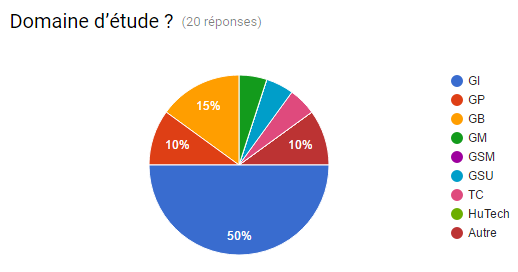
\includegraphics[width=.7\textwidth]{img/sondage_branche}
	\caption{Sondage - Répartition par branches}
\end{figure}
\vspace*{\fill}

On observe que les avis sur les outils déjà existants sont assez mitigés.
En effet, les inconvénients les plus cités sont le manque de personnalisation et le retour en arrière.
D'un autre côté, les avantages cités sont la gratuité et la simplicité d'utilisation.

\newpage
\begin{figure}[!h]
	\centering
	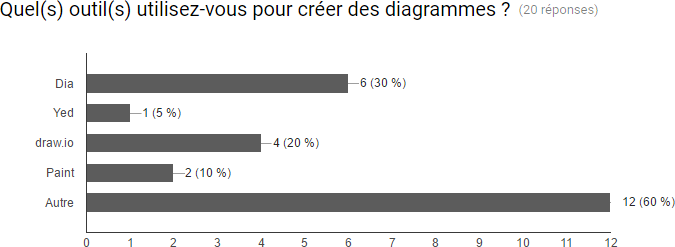
\includegraphics[width=\textwidth]{img/sondage_outils}
	\caption{Sondage - Outils utilisés pour la réalisation de diagrammes}
\end{figure}
\vspace*{\fill}
\begin{figure}[!h]
	\centering
	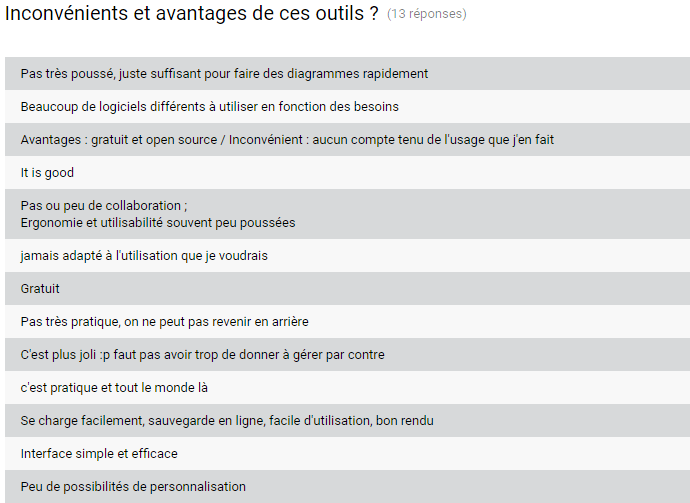
\includegraphics[width=\textwidth]{img/sondage_critique}
	\caption{Sondage - Critiques des outils existants}
\end{figure}
\vspace*{\fill}

\newpage
On peut également voir que les avis quant à l'utilisation d'un appareil mobile pour travailler sont très partagés, on se retrouve à 50\% pour et 50\% contre.
Enfin, l'idée d'une application permettant le travail collaboratif sur appareil mobile est aussi partagée mais tend à pencher pour un avis positif.

\vspace*{\fill}
\begin{figure}[!h]
	\centering
	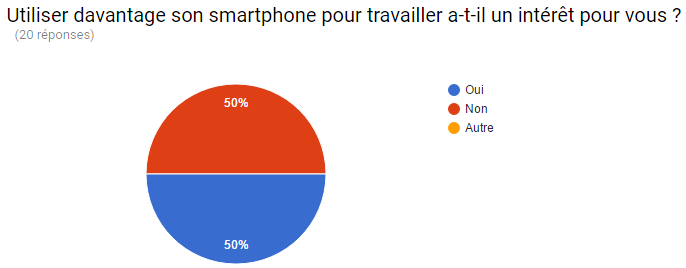
\includegraphics[width=.8\textwidth]{img/sondage_smartphone}
	\caption{Sondage - Critiques des outils existants}
\end{figure}

\vspace*{\fill}
\begin{figure}[h]
	\centering
	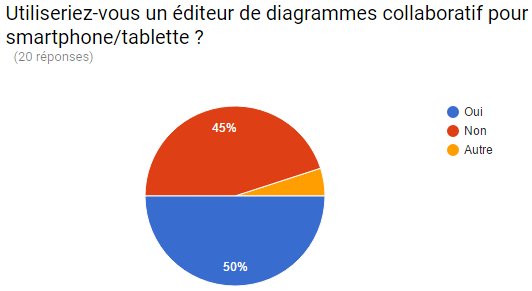
\includegraphics[width=.7\textwidth]{img/sondage_colladia}
	\caption{Sondage - Avis sur Colladia}
\end{figure}
\vspace*{\fill}

\newpage
\subsection{Étude de quelques logiciels concurrents}
Lors de nos recherches, deux applications semblaient réellement en concurrence avec notre solution, à savoir draw.io de Google et DrawExpress de DrawExpress Inc.

\subsubsection{Draw.io}
Néanmoins draw.io, bien que collaboratif n'utilise pas pleinement les fonctionnalités tactiles des supports mobiles.

\vspace*{\fill}
\begin{figure}[h]
	\centering
	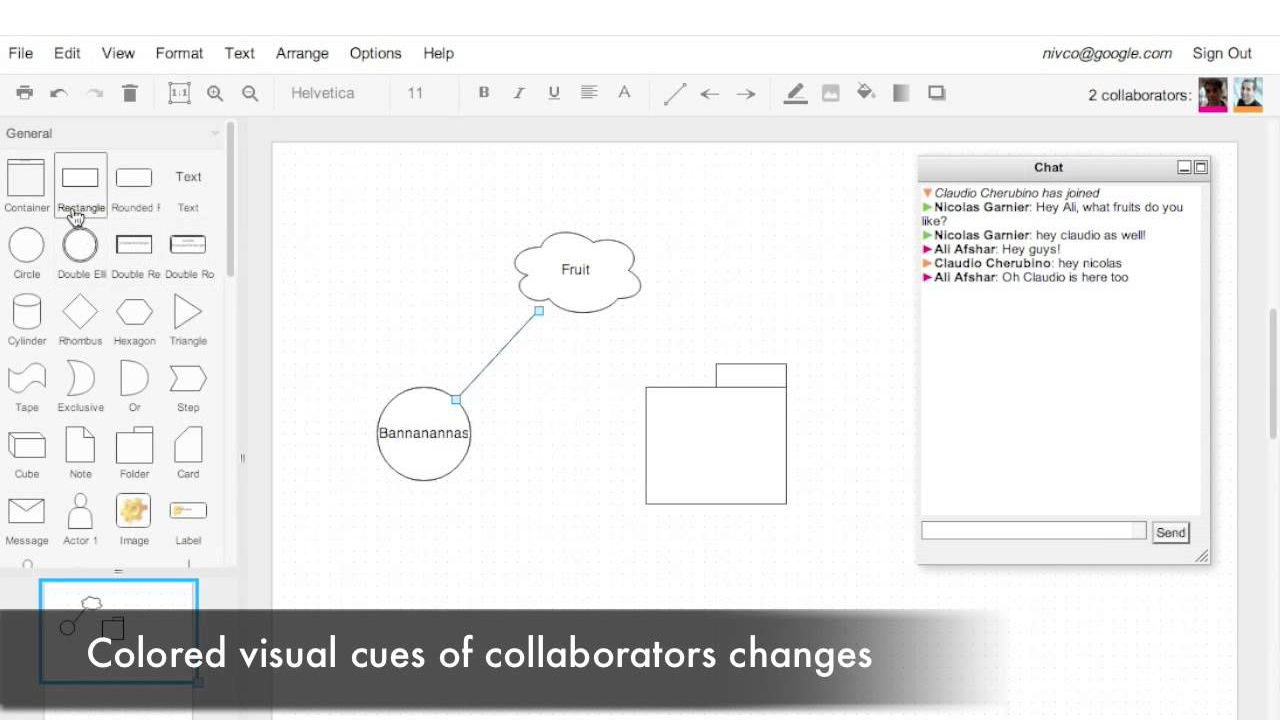
\includegraphics[width=.6\textwidth]{img/drawio}
	\caption{draw.io - Édition en collaboration}
\end{figure}
\vspace*{\fill}

\subsubsection{DrawExpress}
DrawExpress propose un éditeur de diagramme sur mobile.
Il est cross-plateforme (IOS, Android et BlackBerry) mais il ne permet pas de travailler à plusieurs simultanément.

\vspace*{\fill}
\begin{figure}[!h]
	\centering
	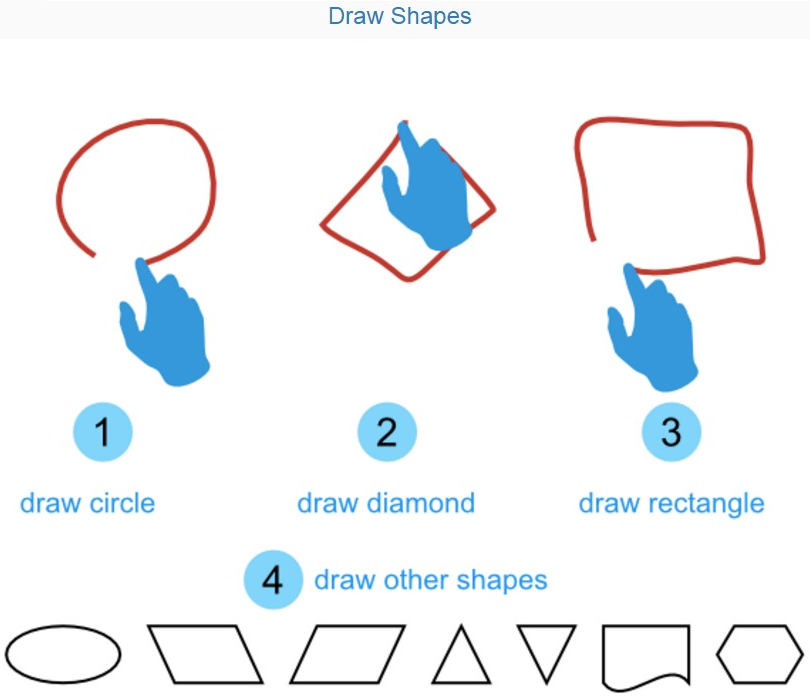
\includegraphics[width=.4\textwidth]{img/DrawExpressRecognition}
	\caption{Aperçu des interactions tactiles de DrawExpress - Reconnaissance de forme}
\end{figure}
\vspace*{\fill}

\newpage
\begin{figure}[!h]
	\centering
	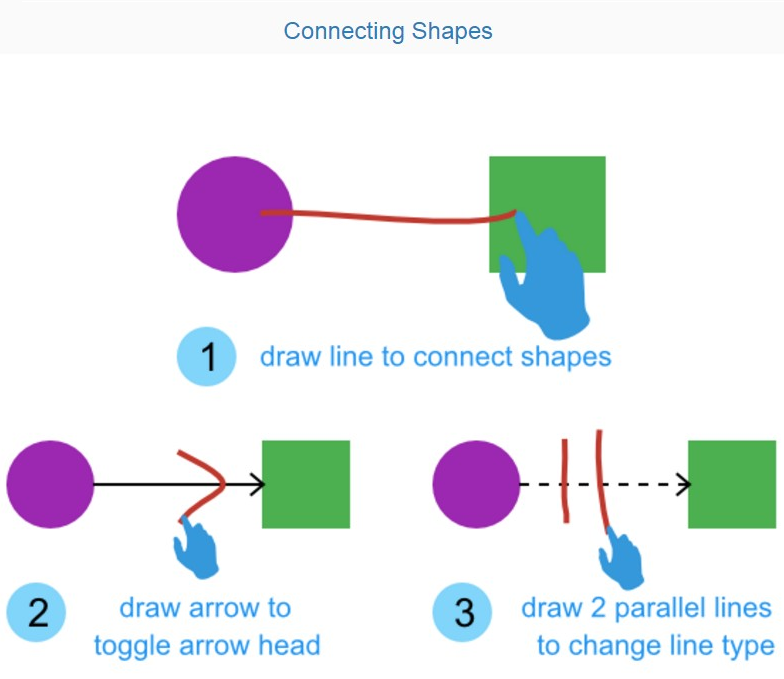
\includegraphics[width=.4\textwidth]{img/DrawExpressLinks}
	\caption{Aperçu des interactions tactiles de DrawExpress - Tracé de lignes}
\end{figure}

Cette application constitue une bonne base d'inspiration pour Colladia puisqu'elle utilise particulièrement les interactions tactiles permises par les smartphones afin de créer, à partir de gestes simples à main levée, des formes prédéfinies qui constituent le diagramme.
De cette manière, l'ergonomie est optimisée pour les écrans tactiles et de petite taille.

\subsubsection{Positionnement}
Le but de Colladia est donc de proposer les deux points forts ces deux logiciels concurrents, à savoir le travail collaboratif et les interactions tactiles.

\newpage
\subsection{Fonctionnalités}
Dans cette partie, on rendra compte des fonctionnalités prévues du cahier des charges, en précisant les modifications qu'elles ont subies lors de leur implémentation.

\subsubsection{Fonctionnalités générales}
La connexion au serveur avec un pseudo a été correctement réalisée : l'utilisateur a la possibilité d'entrer un pseudo et de préciser l'adresse du serveur auquel il faut se connecter pour créer et éditer des diagrammes. Il lui est aussi permis de sélectionner une couleur personnalisée.

Dans la vue listant les diagrammes, il suffit de sélectionner le diagramme voulu et de cliquer sur "Access" pour le rejoindre. Il est aussi possible de supprimer le diagramme.
		
		\vspace*{\fill}
		\begin{figure}[!h]
			\centering
			\begin{subfigure}[t]{.3\textwidth}
				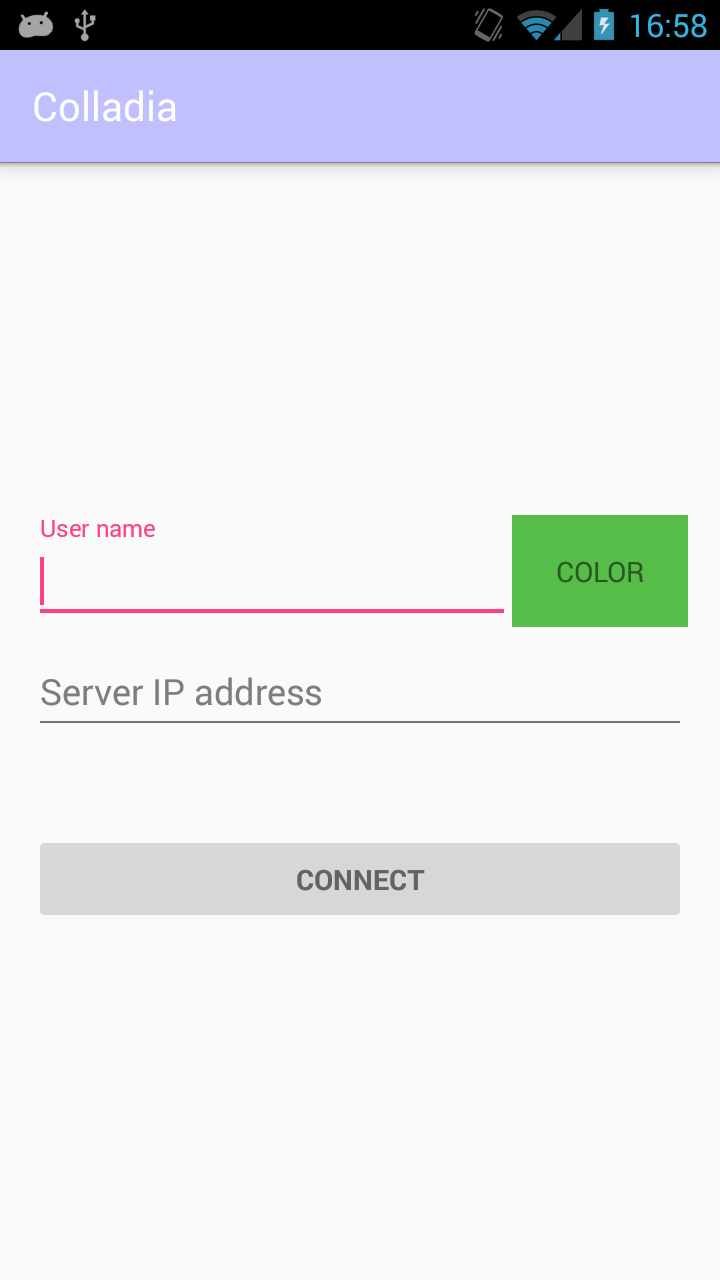
\includegraphics[width=\textwidth]{img/screen/new/colladia_connexion}
				\subcaption{Connexion}
			\end{subfigure}
			~
			\begin{subfigure}[t]{.3\textwidth}
				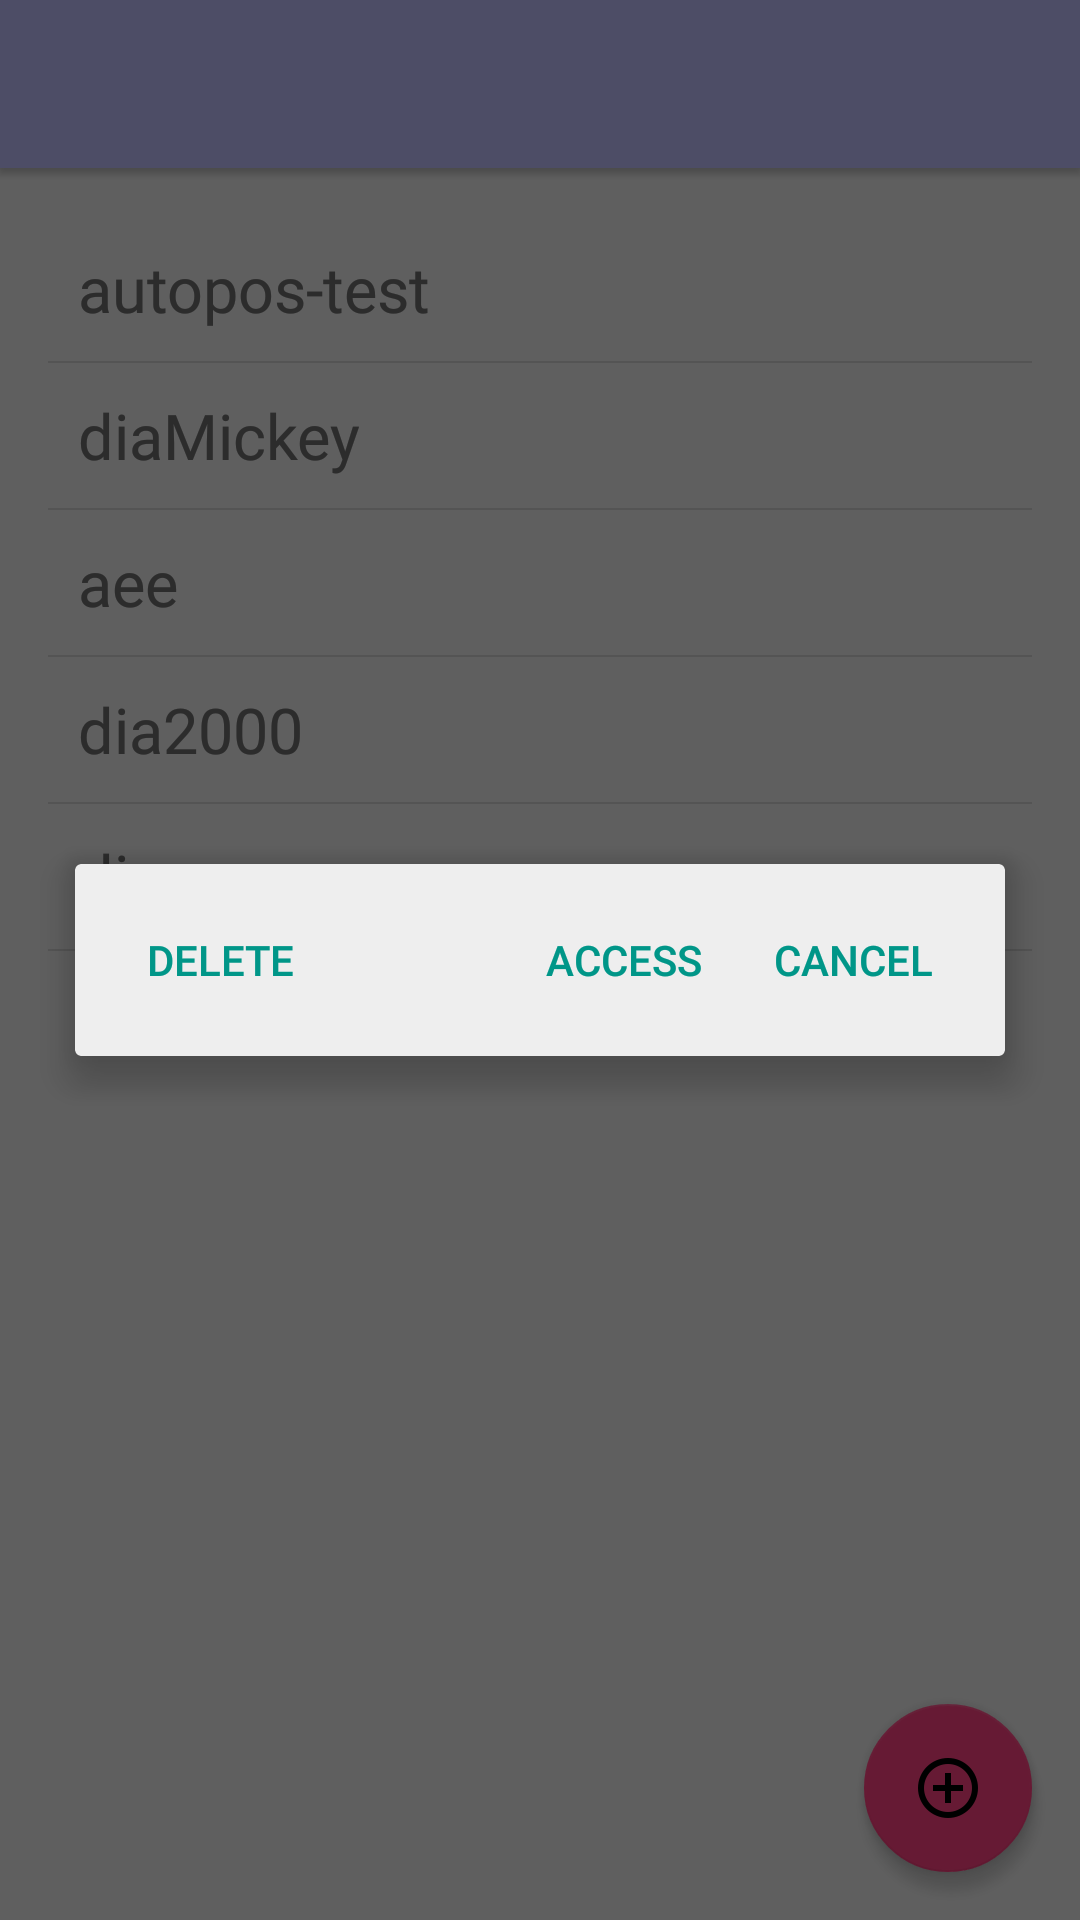
\includegraphics[width=\textwidth]{img/screen/colladia_workspaces_select}
				\subcaption{Liste des diagrammes}
			\end{subfigure}
			~
			\begin{subfigure}[t]{.3\textwidth}
				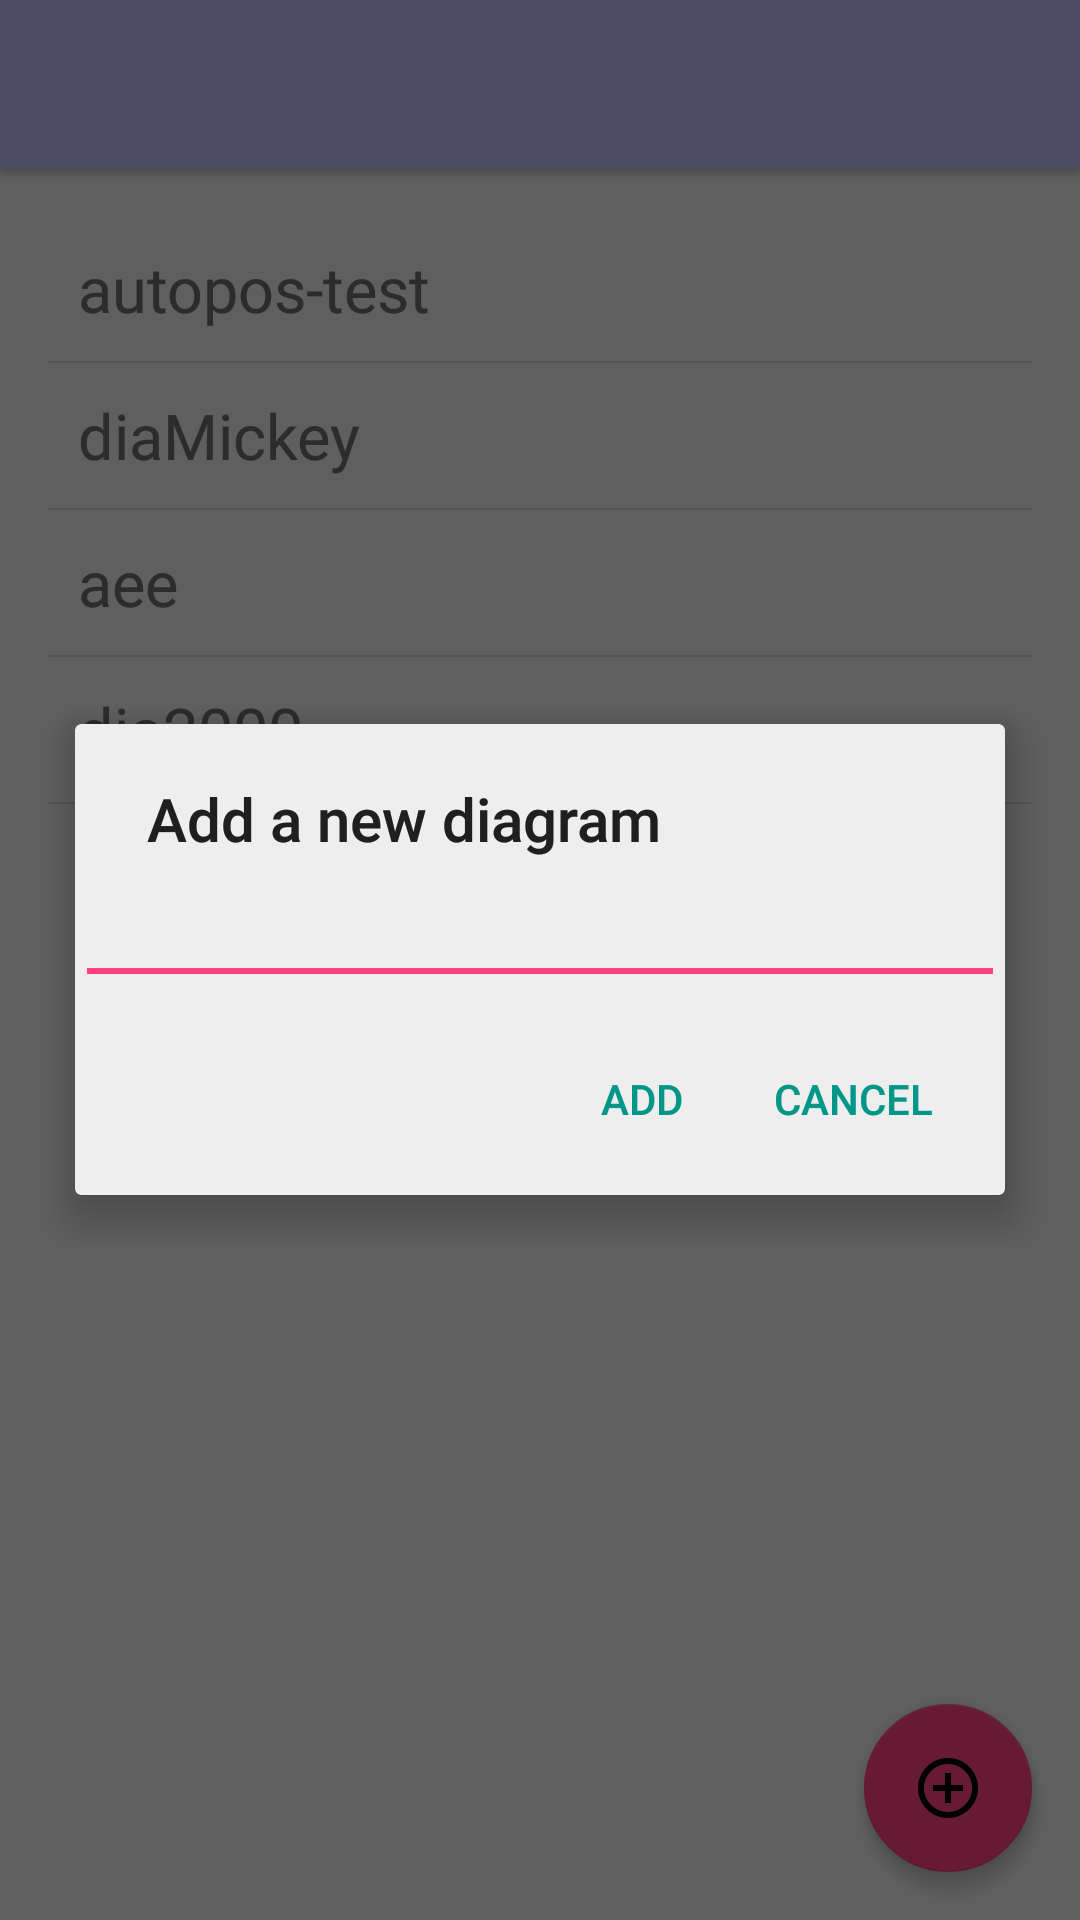
\includegraphics[width=\textwidth]{img/screen/colladia_create_workspace}
				\subcaption{Création}
			\end{subfigure}
			\caption{Colladia - Connexion à l'application et sélection d'un diagramme}
		\end{figure}
		\vspace*{\fill}
		
Inspiré des mouvements de déplacements habituels sur les interfaces tactiles, le mouvement de \textit{swipe} permet de déplacer la vue. Il est aussi possible d'utiliser le mouvement de \textit{pinch} pour effectuer un zoom.

La prochaine partie expose et détaille les différentes fonctionnalités d'ajout, de manipulation, et d'édition des éléments d'un diagramme.
	
\newpage
\subsubsection{Fonctionnalités tactiles implémentées}
Une icône est toujours présente et visible dans le coin supérieur droit de l'application. Elle propose les mêmes items de création et édition que le menu contextuel principal, en ajoutant la possibilité de revenir à la liste des diagrammes disponibles.

Un menu contextuel circulaire apparaît après un appui long sur l'espace de travail. Depuis celui-ci, on sélectionne et crée des formes prédéfinies (Classes UML, cercles, carrés, rectangles), on recentre l'espace de travail, et on repositionne les éléments pour éviter les chevauchements.

Un appui long sur un élément permet d'ouvrir un menu contextuel spécifique à l'élément, qui permet de le dupliquer, de le supprimer, ou bien encore d'effacer les liens dont il est l'origine.

		\vspace*{\fill}
		\begin{figure}[!h]
			\centering
			\begin{subfigure}[t]{.3\textwidth}
				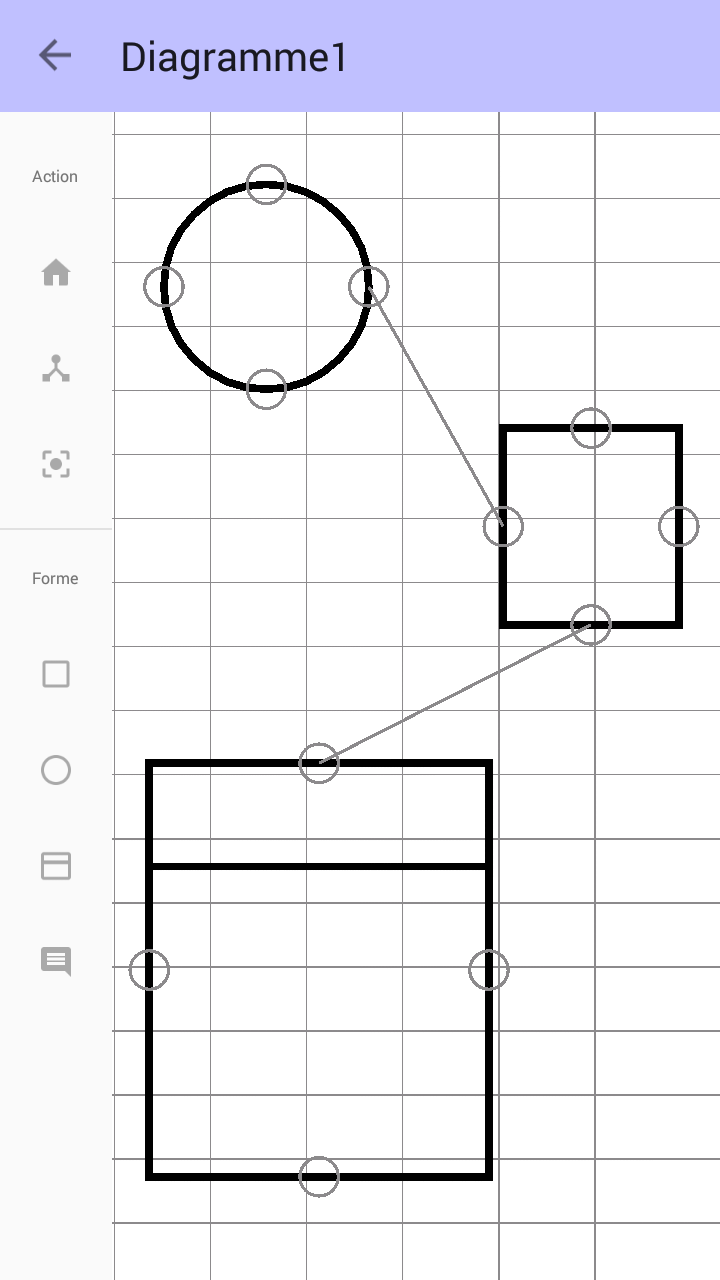
\includegraphics[width=\textwidth]{img/screen/new/colladia_draw_view_menu_main}
				\subcaption{Menu latéral}
			\end{subfigure}
			~
			\begin{subfigure}[t]{.3\textwidth}
				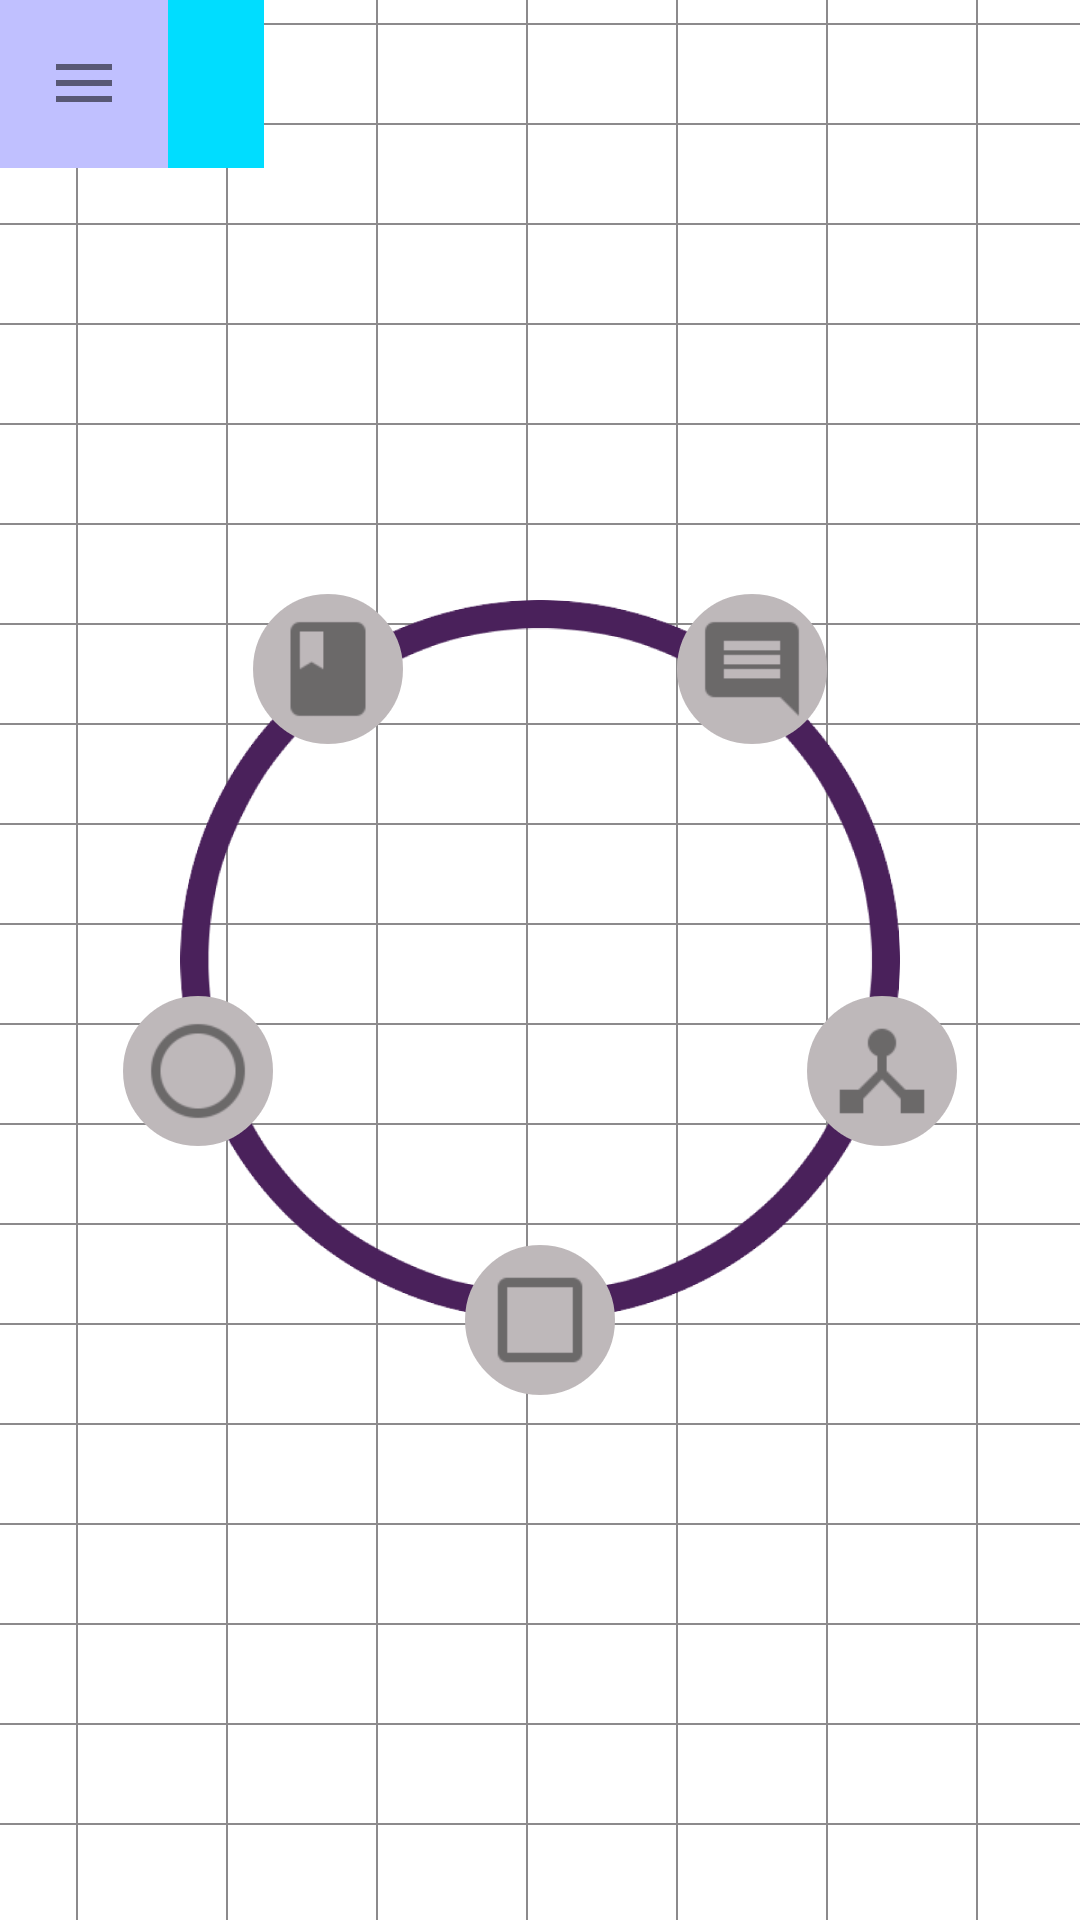
\includegraphics[width=\textwidth]{img/screen/colladia_draw_view_menu_contextuel_main}
				\subcaption{Menu contextuel principal}
			\end{subfigure}
			~
			\begin{subfigure}[t]{.3\textwidth}
				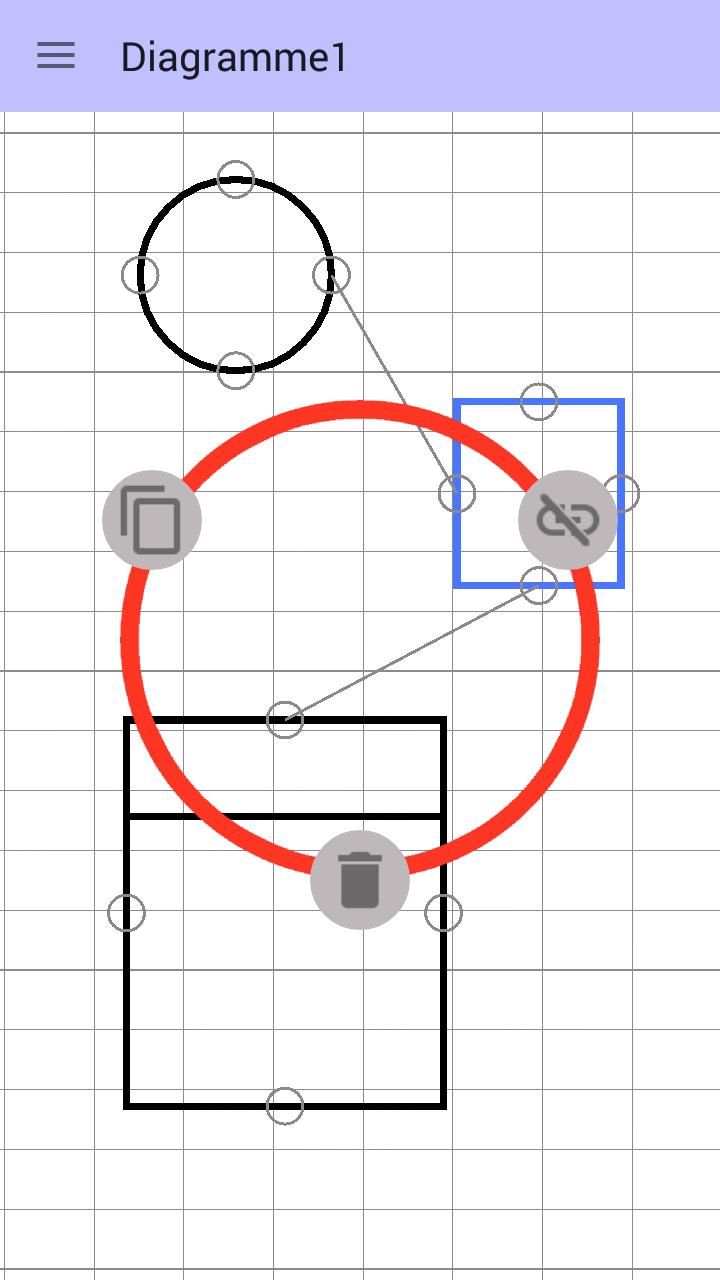
\includegraphics[width=\textwidth]{img/screen/new/colladia_draw_view_menu_contextuel_select}
				\subcaption{Menu contextuel de selection}
			\end{subfigure}
			\caption{Colladia - Menu latéral et menus contextuels}
		\end{figure}
		\vspace*{\fill}

Un \textit{double-tap} sur un élément permet d'insérer du texte dans la forme.

Un mouvement de \textit{slide} permet de se déplacer sur la zone de dessin. Si un élément est sélectionné alors on déplace ce dernier.

Un appui sur un élément le sélectionne et le colore de la couleur de l'utilisateur. En appuyant de nouveau sur un autre élément ou sur un espace vide, on dé-sélectionne l'élément, et il reprend sa couleur normale.

\newpage
		\begin{figure}[!h]
			\centering
			\begin{subfigure}[t]{.27\textwidth}
				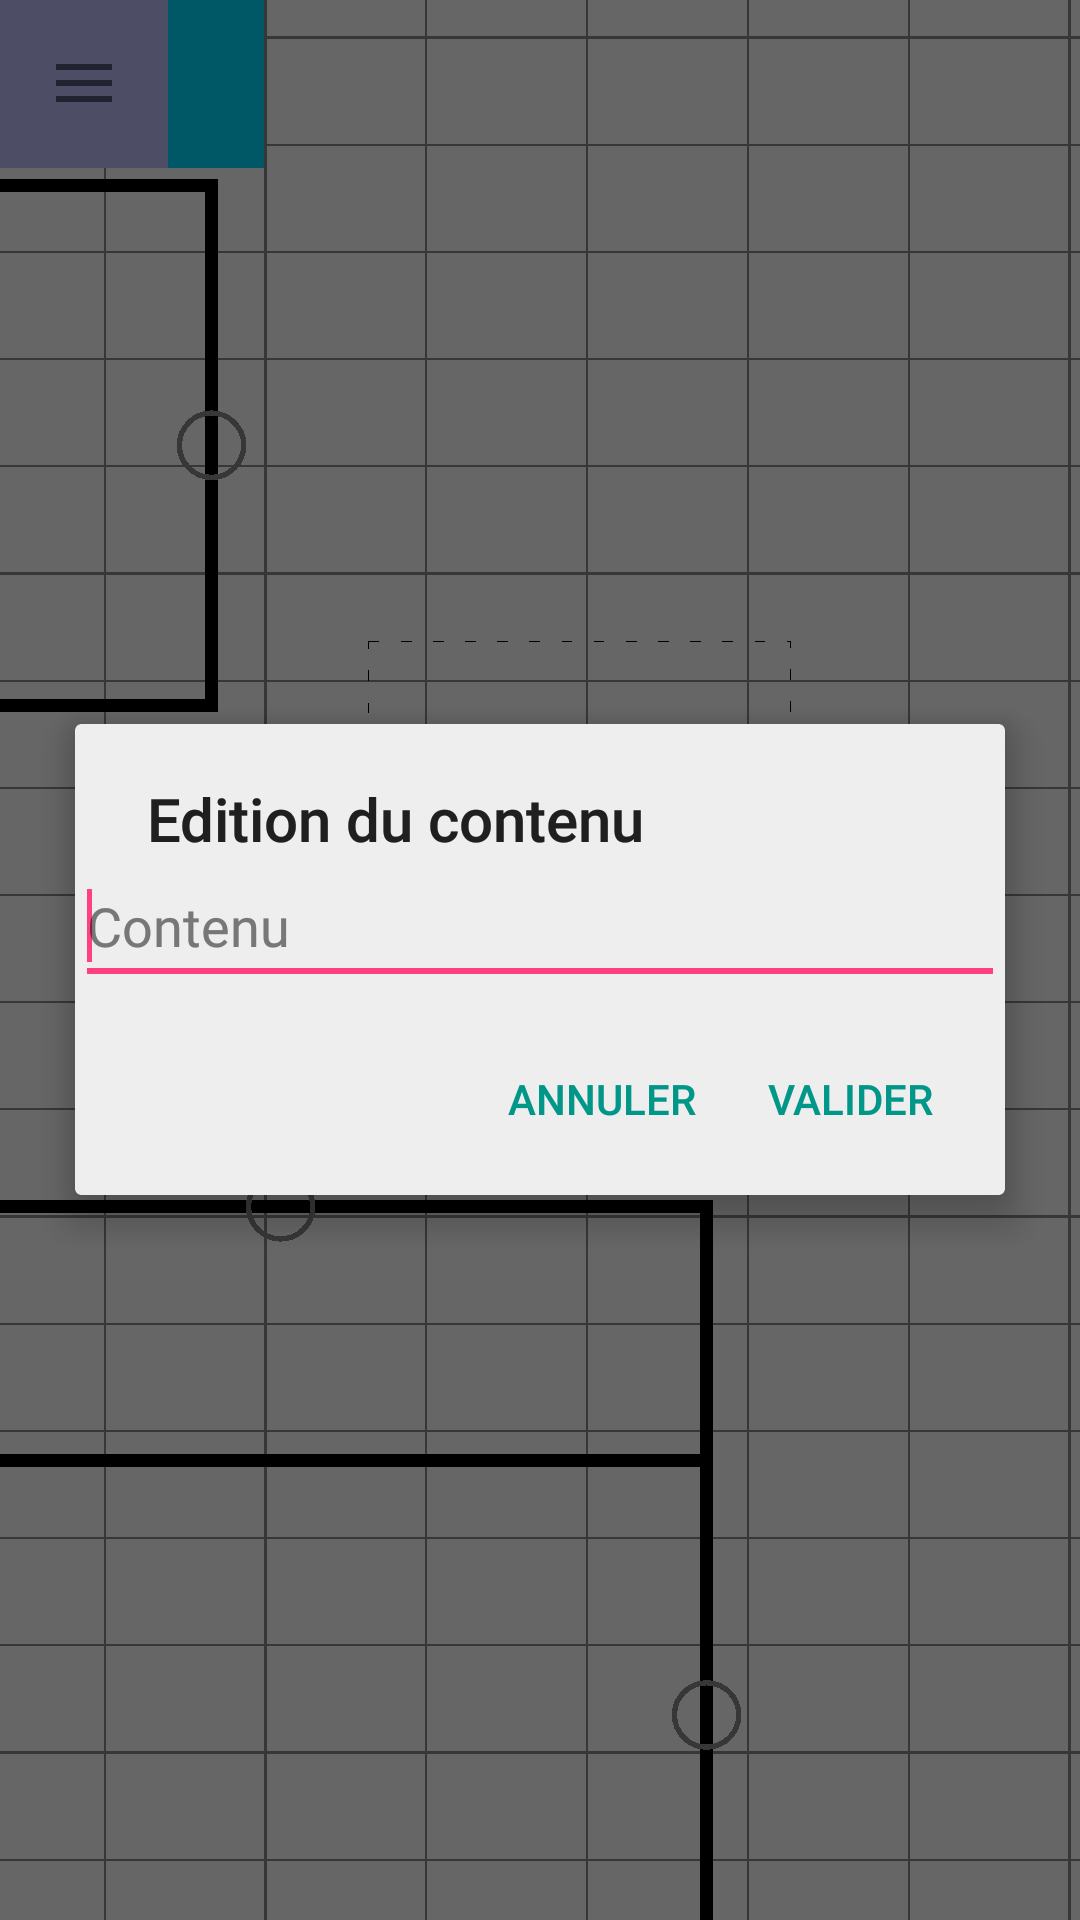
\includegraphics[width=\textwidth]{img/screen/colladia_draw_view_element_change_text}
				\subcaption{Ajout de texte dans un élément}
			\end{subfigure}
			~
			\begin{subfigure}[t]{.27\textwidth}
				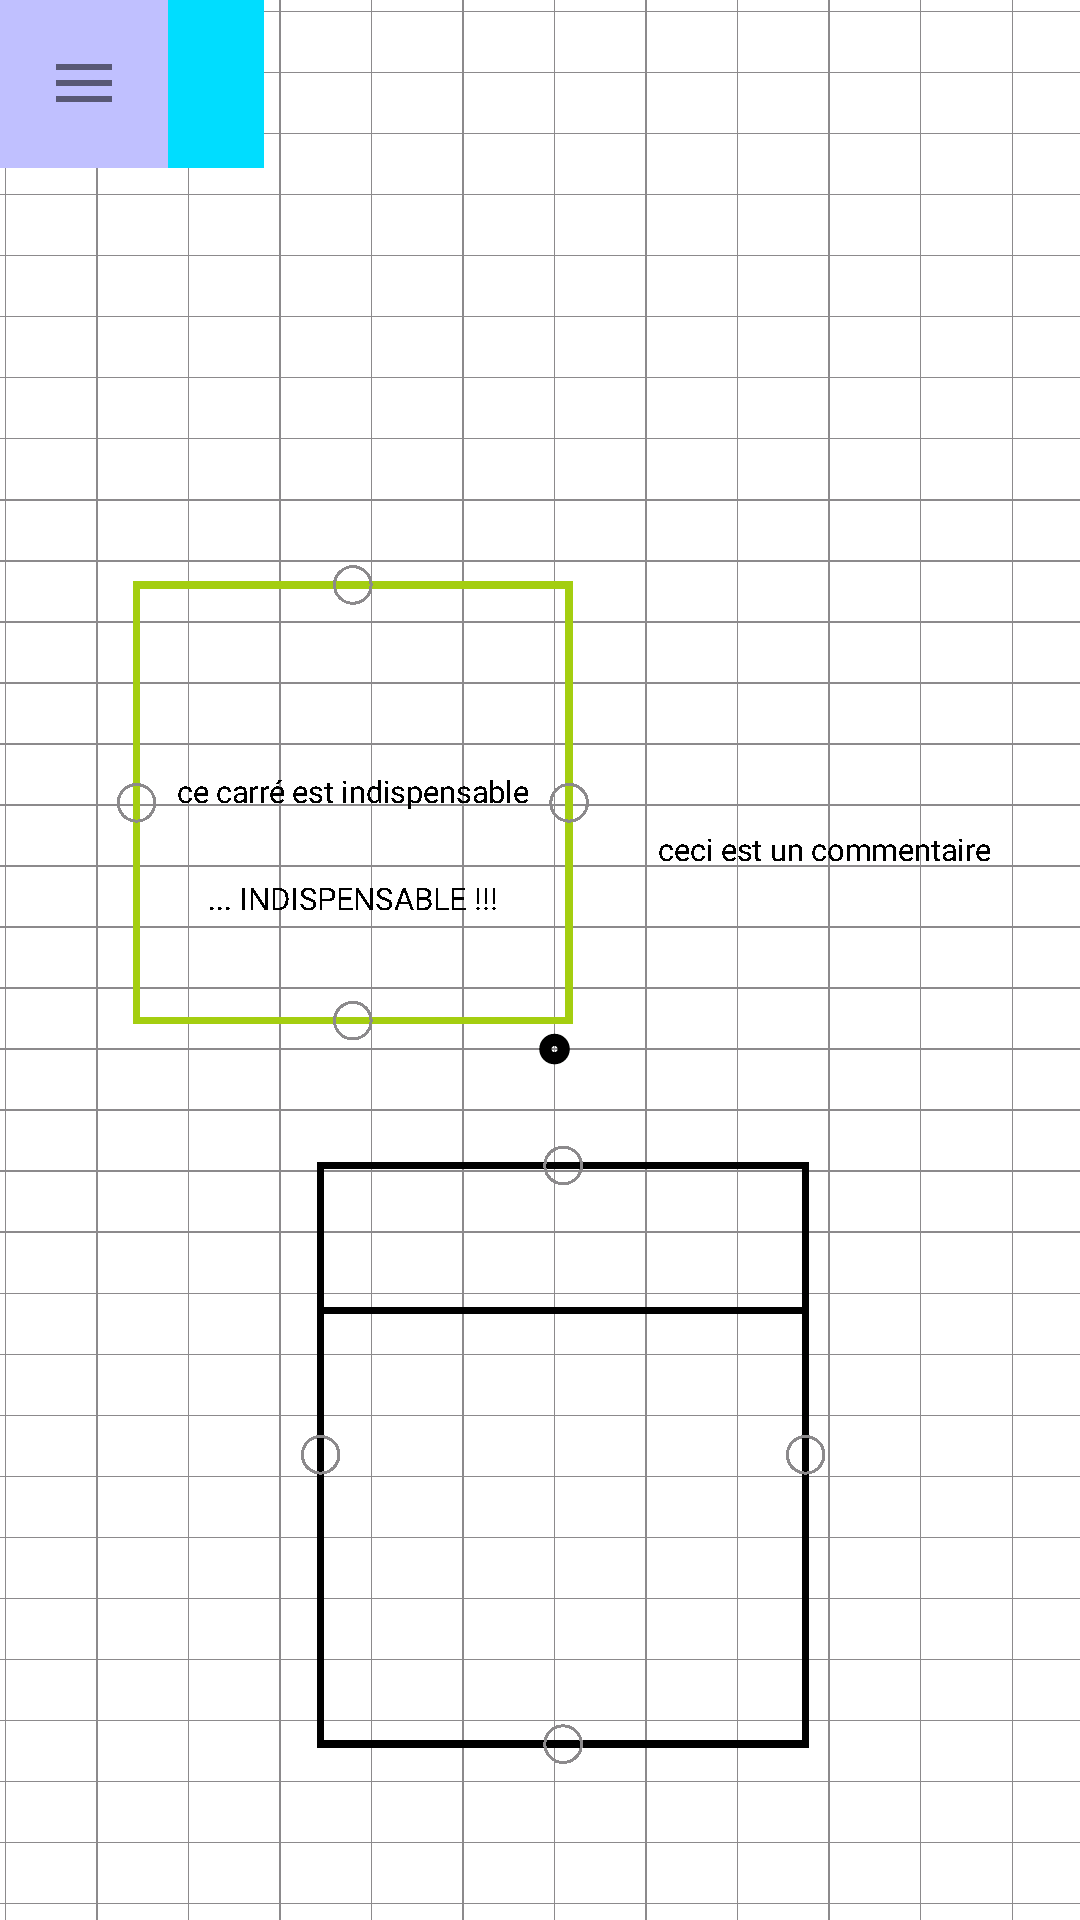
\includegraphics[width=\textwidth]{img/screen/colladia_draw_view_element_text}
				\subcaption{Selection}
			\end{subfigure}
			\caption{Colladia - Ajout de texte et sélection d'élément}
		\end{figure}
		\vspace*{\fill}
		
Le mouvement de \textit{pinch} habituel est reconnu par l'application. Lorsqu'il est appliqué sur un élément, il implique son redimensionnement. Sinon, il permet de gérer le niveau de zoom sur la zone de travail.

Pour pouvoir représenter des flux ou relations dans les diagrammes, l'utilisateur peut sélectionner les ancres, qui sont au nombre de 4 pour chaque élément, puis en restant appuyé sur l'écran et en rejoignant une seconde ancre un lien sera créé.

	\vspace*{\fill}
		\begin{figure}[!h]
			\centering
			\begin{subfigure}[t]{.27\textwidth}
				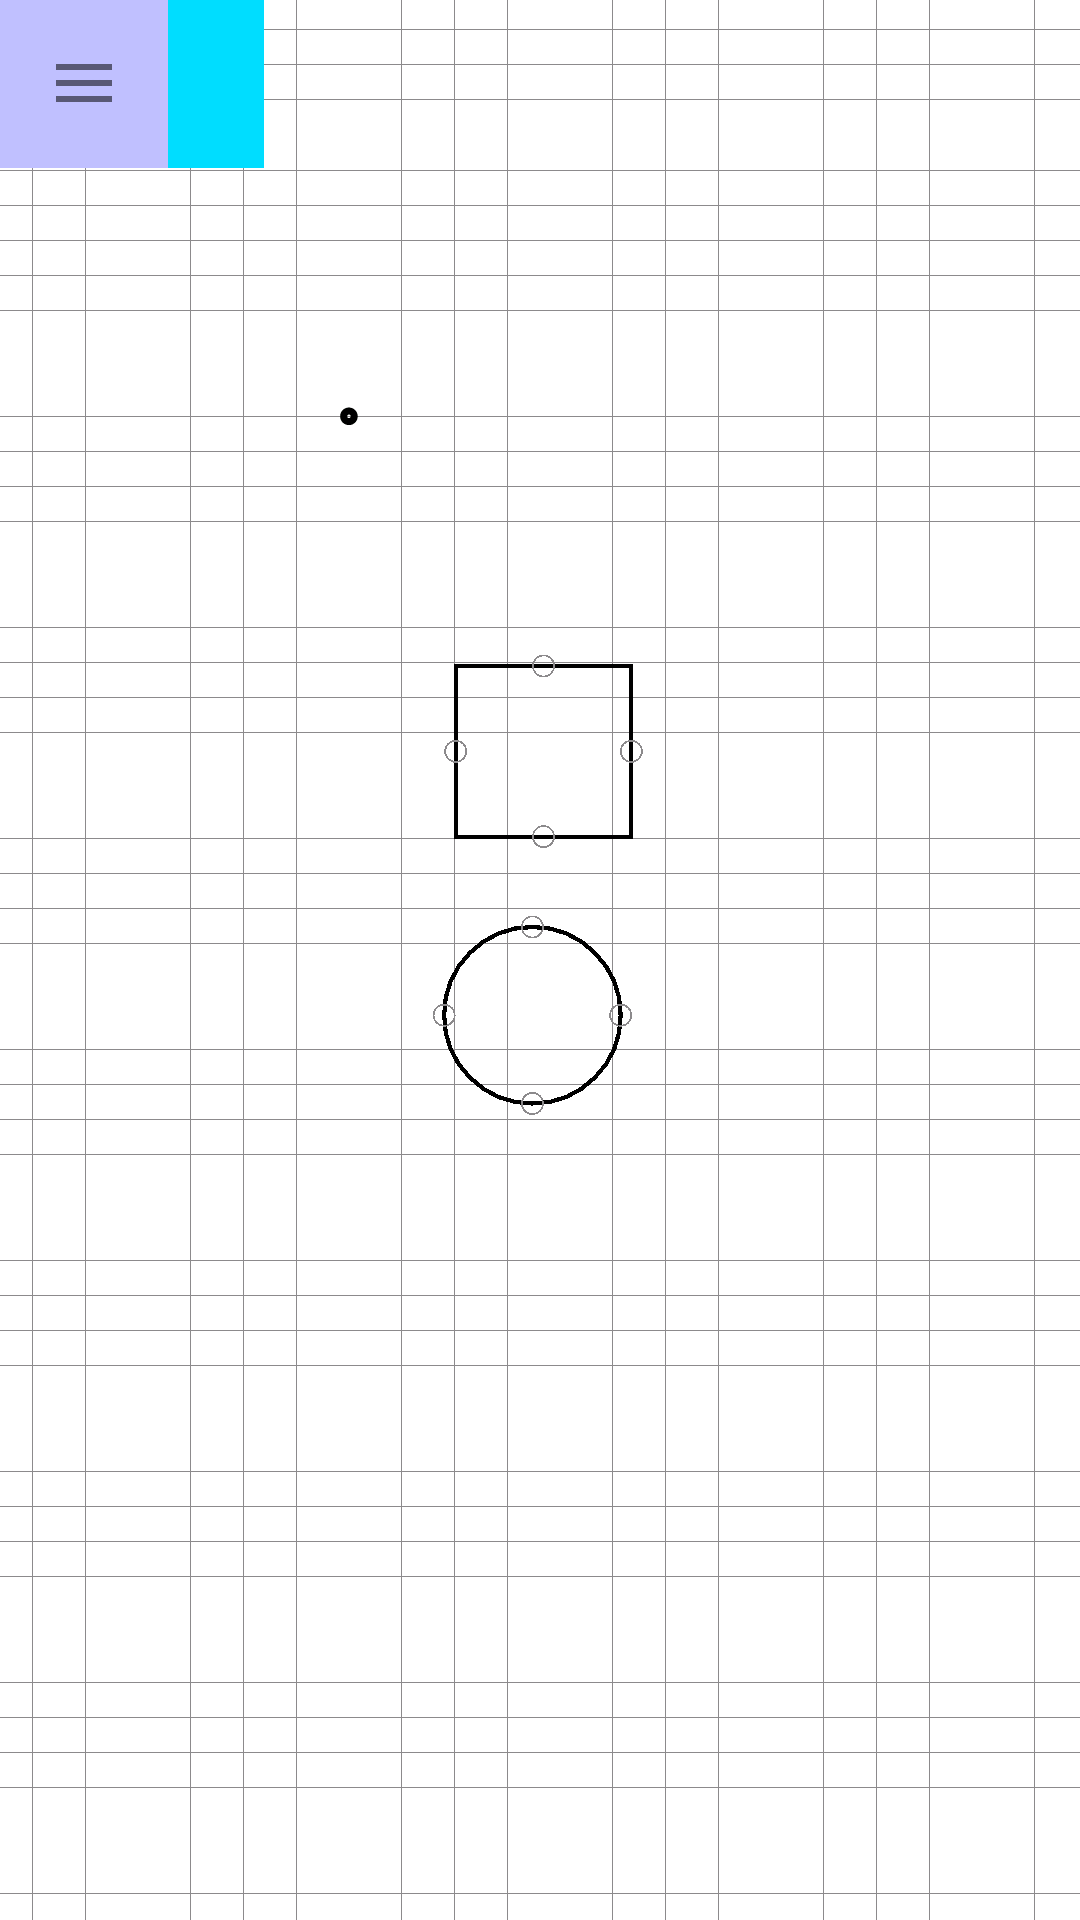
\includegraphics[width=\textwidth]{img/screen/colladia_draw_view_zoom_out}
				\subcaption{Zoom arrière}
			\end{subfigure}
			~
			\begin{subfigure}[t]{.27\textwidth}
				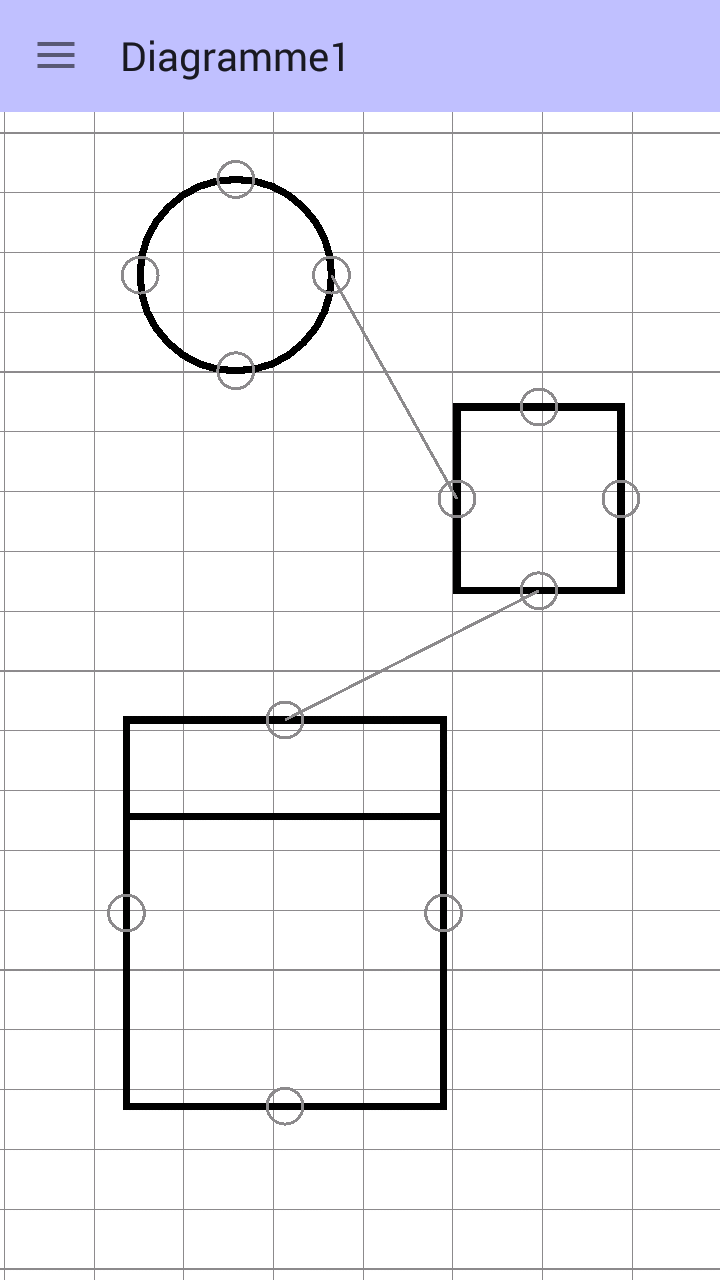
\includegraphics[width=\textwidth]{img/screen/new/colladia_draw_view_element_links}
				\subcaption{Liens}
			\end{subfigure}
			\caption{Colladia - Zoom et liens entre les éléments}
		\end{figure}

L'espace de travail est virtuellement infini. Ainsi, il est plutôt facile de se perdre et de ne pas retrouver les éléments créés. Afin de pallier à ce problème d'utilisabilité, un item du menu contextuel principal permet de recentrer la vue sur l'origine.

Un autre item de ce menu contextuel permet d'effectuer une requête au serveur pour attribuer une nouvelle position à tous les éléments en évitant les chevauchements. Toutefois, cette méthode ne prend pas encore en compte les liens qui peuvent relier certains éléments.

\subsubsection{Fonctionnalités non-implémentées}
Dans la version actuelle de l'application, la gestion des collaborateurs n'est pas effectuée.
Il n'est donc pas possible de voir les vues des collaborateurs, ni de connaître la liste des utilisateurs connectés à un instant précis.

Néanmoins lorsqu'un élément est sélectionné, il prend la couleur spécifique de l'utilisateur.

Ainsi il est possible de déterminer lorsqu'un item est modifié par un collaborateur. 
La gestion des différents niveaux de plans n'est pas proposé, ainsi que le fait d'attirer l'attention de l'utilisateur sur un élément en particulier, même si cette fonctionnalité est retrouvé lorsque l'on sélectionne l'élément, ce qui le colore. 

\subsubsection{Développements supplémentaires envisagés}
Voici les fonctionnalités optionnelles pour améliorer l'expérience utilisateur qui avaient été proposées au début du projet :
\begin{itemize}
\item un chat pour laisser la possibilité aux membres de communiquer
\item l'utilisation de commandes vocales pour faciliter l'utilisation de l'application
\item un système de commentaire sur les diagrammes, pour fournir des informations complémentaires
\item une fonction de recherche de texte
\item la fusion de diagrammes
\item l'exportation des diagrammes sous différents formats (graphml par exemple)
\item la gestion des utilisateurs
\item la possibilité de restreindre l'accès à un diagramme par un mot de passe
\item la gestion des sauvegardes hors-ligne
\item le dessin à main levé qui permet une reconnaissance de forme et d'ajout d'élément automatiquement
\end{itemize}

Parmi ces dernières la gestion des sauvegardes automatiques côté serveur a été implémenté, en sauvegardant dans des fichiers les diagrammes sous format JSON. Les diagrammes sont donc persistants et accessibles d'une utilisation à l'autre.

\newpage
\subsection{Technologies}
Concernant les technologies employées, le serveur utilise la plateforme multi-agent JADE et communique avec le client via une API Restlet.
Côté client il avait été envisagé de réaliser l'application en utilisant Xamarin dans un premier temps, néanmoins la technologie ne fonctionnait pas correctement chez tous les membres du projet.
Il a fallu réagir et prendre une décision pour pouvoir réaliser le projet dans le délai imparti.
Le choix a été pris de réaliser l'application en Android natif, ce qui permet d'avoir accès à une documentation importante et d'avoir une application réactive.
\vspace*{-.5cm}

\subsection{Architecture de l'application}
L'application cliente est constituée de 3 vues principales, qui s'occupent de l'essentiel des interactions avec l'utilisateur.
Elles permettent de gérer les entrées d'utilisateurs.
La première vue gère la connexion au serveur avec la création des données utilisateurs. Lors de la connexion, la deuxième vue est affichée pour lister les diagrammes existants et en créer de nouveau.
Une fois un diagramme sélectionné, la dernière vue est affichée pour permettre d'éditer le diagramme. 
	
 	\vspace*{\fill}
	\begin{figure}[!h]
		\centering
		\includegraphics[width=.7\textwidth]{img/FlowAppli}
		\caption{Colladia - Vues principales}
	\end{figure}
 	\vspace*{\fill}
\vspace*{-.5cm}

\subsubsection{Architecture Générale}
L'application peut-être schématisée comme suit, à savoir le contrôleur situé entre la vue et le modèle. Dès qu'une modification est effectuée au niveau de la liste des éléments du modèle le contrôleur met à jour la vue.
Dans le sens contraire lorsque l'utilisateur interagit avec la vue une requête est envoyé au serveur pour mette à jour le diagramme sur le serveur pour les autres utilisateurs.
Le modèle est mis à jour par le serveur par le retour d'une requête de modification ou par la réponse d'une requête GET qui est réalisé périodiquement pour savoir si de nouvelles modifications sont présentes sur le serveur.

 	\vspace*{\fill}
	\begin{figure}[!h]
		\centering
		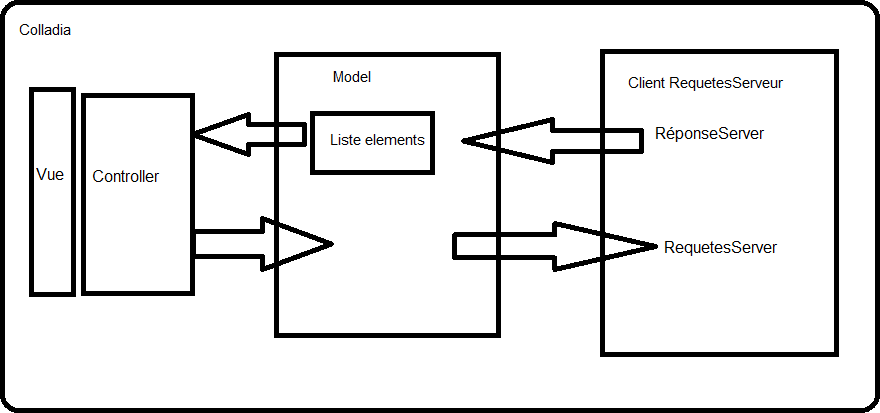
\includegraphics[width=.6\textwidth]{img/archiGeneral}
		\caption{Colladia - Schéma de l'architecture général}
	\end{figure}
 	\vspace*{\fill}
	
\newpage
\subsubsection{Structure de données}
Outre les données utilisateur, les structures de données principales concernent les éléments.
Pour pouvoir proposer de nombreuses formes prédéfinis, il a été décidé de créer une classe Element abstraite dont hériteraient toutes les formes.
Ainsi le contrôleur peut gérer les éléments sans avoir à connaître le type d'élément dont il s'agit.
Ce polymorphisme induit un couplage plus léger et permet donc une plus grande souplesse du contrôleur.
Certaines méthodes telles que \lstinline$isTouch(PointF indexUser)$ qui permet de savoir si un élément a été touché par l'index de l'utilisateur ou \lstinline$draw()$ qui permet de dessiner l'élément.
En surchargeant ces différentes méthodes chaque forme peut proposer un comportement différent.
Les éléments se distinguent entre eux par le stockage d'un identifiant \lstinline$UUID$ qui est unique, ce qui permet de sérialiser/dé-sérialiser sous format JSON les objets puis retrouver leurs références.

Chaque élément possède 4 ancres (Top, Bottom, Left, Right) qui permettent de lier les éléments entre eux.
Pour ce faire chaque ancre possède l'UUID de son parent ainsi que celui de l'ancre auquel il est associé.
Lors de la sérialisation/dé-sérialisation des éléments il est possible de retrouver l'ancre associée sans pour autant avoir une référence sur l'objet constamment.

\subsubsection{Gestion des données}
Le singleton \lstinline$Manager$ propose des méthodes telles que \lstinline$changeText(Element elmnt, Text text)$ qui permet dans un premier temps de changer le texte l'élément, puis demande au \lstinline$Requestator$ d'envoyer une requête au serveur pour y mettre à jour l'élément.
Le singleton \lstinline$Requestator$ s'occupe de réaliser les requêtes au serveur en utilisant le framework android Volley.
Le modèle possède le diagramme couramment modifié ainsi que l'horloge logique utilisé par le serveur pour renvoyer les dernières modifications effectuées.

La classe \lstinline$ElementFactory$ permet de générer les éléments spécifiques tels un Cercle ou un Rectangle pour les proposer au Manager qui via le polymorphisme traitera l'objet comme un simple \lstinline$Element$.

\subsubsection{Différentes vues}
On retrouve le concept du MVC au niveau des différentes vues que ce soit au niveau de la connexion au serveur avec les données utilisateur, mais aussi avec la liste des diagrammes qui met à jour automatiquement la vue lorsqu'une modification arrive du serveur et modifie le modèle. Le design pattern Observable était une nécessité dans le contexte asynchrone de requêtage HTTP.

% \paragraph{Édition d'un diagramme}
Concernant la zone de dessin il a fallu mettre en place une sorte de machine à états qui changerait de "mode" selon les interactions de l'utilisateur. Il existe différents modes (\lstinline$ZOOM$, \lstinline$SCROLL$, \lstinline$INSERT$, ...), ce qui permet de déterminer le comportement à adopter selon la situation rencontrée.

La méthode \lstinline$onTouchEvent()$ réagit aux différentes interactions de l'utilisateur, puis appelle la méthode adéquate comme par exemple \lstinline$moveTouch()$ qui correspond au déplacement du doigt de l'utilisateur sur l'écran.

\newpage
	\begin{figure}[!h]
		\centering
		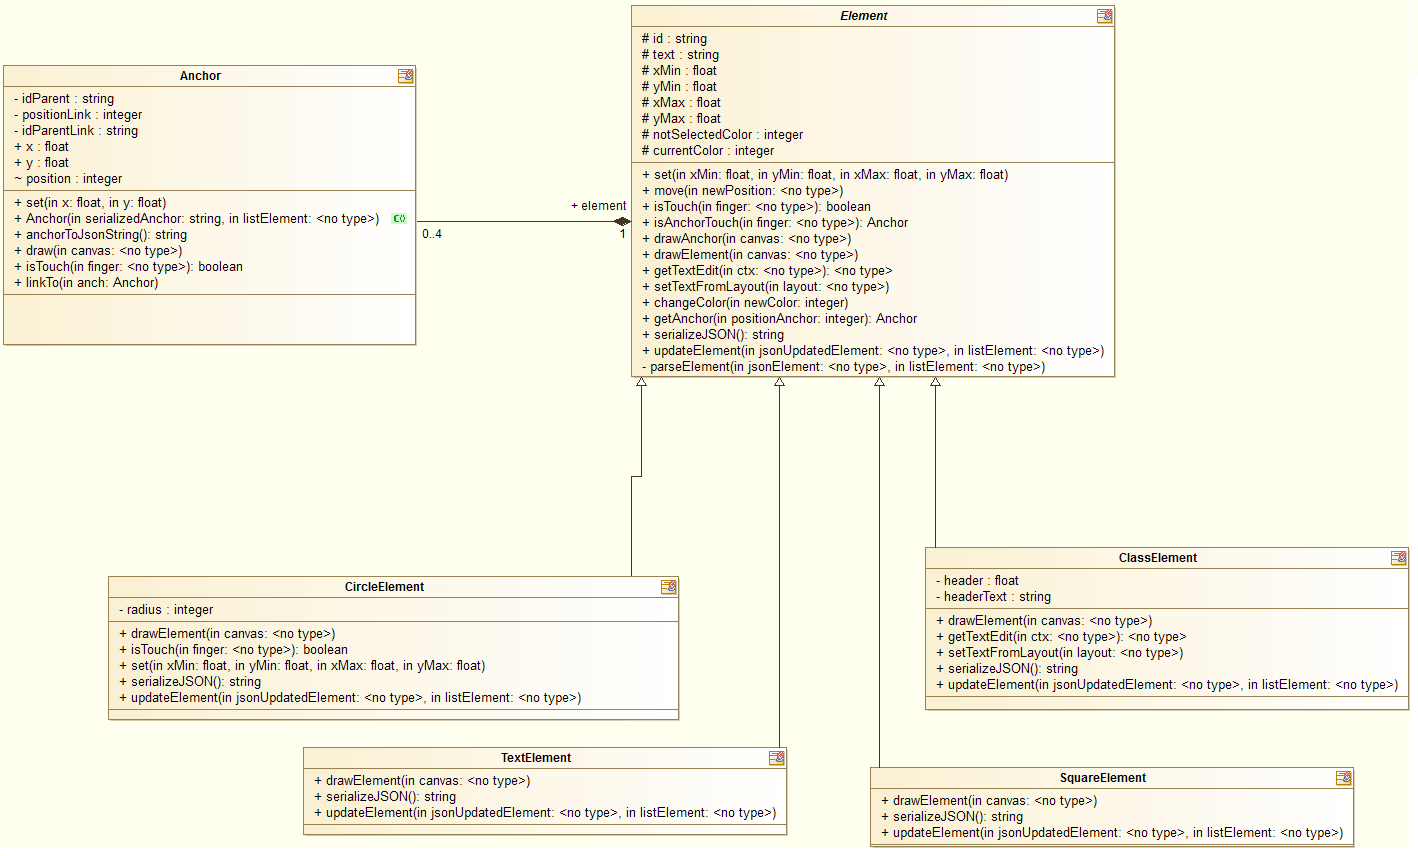
\includegraphics[width=\textwidth]{img/UmlArchiStructureData}
		\caption{Colladia - Structure de données simplifiée}
	\end{figure}

\newpage
	\begin{figure}[!h]
		\centering
		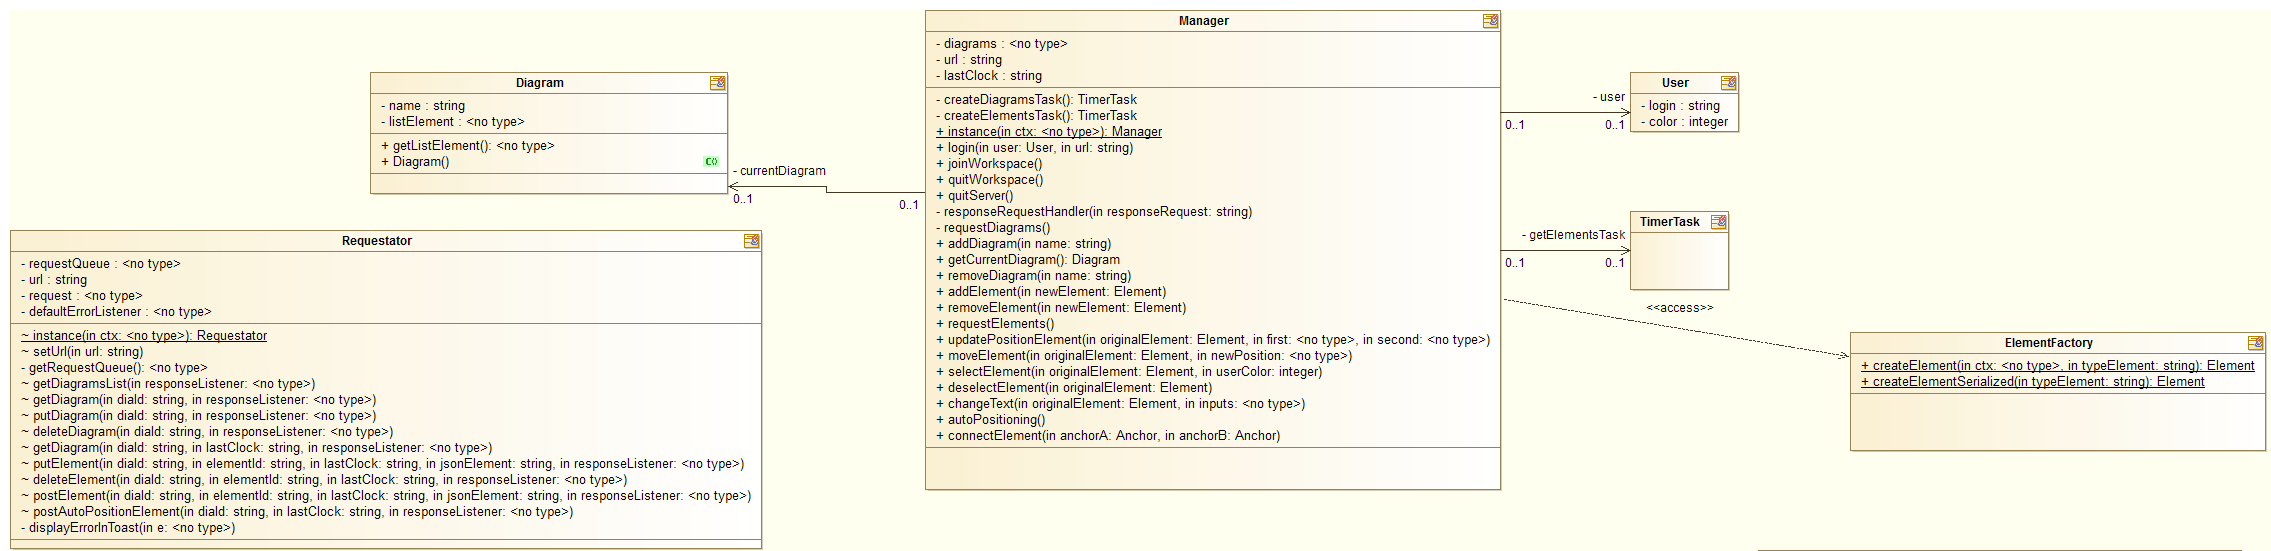
\includegraphics[width=.9\textwidth]{img/UmlArchiGeneral}
		\caption{Colladia - Gestion des données simplifiée}
	\end{figure}

\newpage
	\begin{figure}[!h]
		\centering
		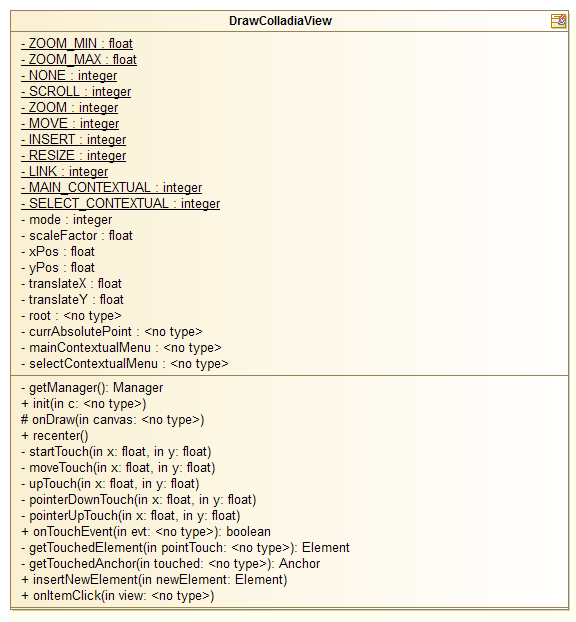
\includegraphics[width=.8\textwidth]{img/UmlDrawView}
		\caption{Colladia - DrawColladiaView}
	\end{figure}

\subsection{Limites et améliorations}
L'application possède une base intéressante et fonctionnelle, cependant on peut citer quelques limites principales.
La première limite étant le nombre restreint d'éléments différents qui sont actuellement proposés.
Un travail important été réalisé pour factoriser un maximum de code des éléments au niveau de la classe \lstinline$Element$, ce qui permet de créer assez facilement des formes diverses et variés.
Une des fonctionnalités supplémentaires qui pourrait aider l'utilisateur serait de permettre une sélection groupée, en plus des différentes fonctionnalités optionnelles décrites auparavant.

\newpage
\section{Serveur multi-agent}
\subsection{Description générale du système}
Le serveur multi-agent a pour but de permettre la dimension collaborative de Colladia.
C'est en effet son rôle d'informer les différents clients éditant un même diagramme des modifications effectuées par les autres utilisateurs.
D'un point de vue technique, le serveur utilise un certain nombre de technologies :
\begin{itemize}
	\item Les requêtes des clients sont reçues via une interface REST implémentée grâce au framework Java Restlet. Cette technologie étant par définition unidirectionnelle, les clients doivent effectuer des requêtes régulières sur le serveur pour être tenus au courant des modifications du diagramme.
	\item Le traitement des requêtes est effectué par un système multi-agent utilisant le framework JADE.
	\item Le contenu des requêtes REST et des messages du SMA sont sérialisés en JSON via la librairie Java Jackson.
\end{itemize}
~\\
La structure du SMA est divisée en deux conteneurs :
\begin{itemize}
	\item Le conteneur principal où résident notamment les agents standards JADE (DF, AMS, etc.) ainsi que l'agent lié au serveur Restlet qui va transformer les requêtes REST reçues en messages pour le SMA (RestAgt). On y trouve aussi l'agent chargé de sauvegarder régulièrement l'état des différents diagrammes dans des fichiers de manière à pouvoir restaurer leur état après un éventuel redémarrage du serveur (SaveAgt).
	\item Le conteneur de diagramme contenant pour chaque diagramme :
	\begin{itemize}
		\item Un ou plusieurs agents élément représentant le diagramme en soi ou des éléments présents dans ce dernier (EltAgt). Ces agents forment entre eux une arborescence dont l'élément représentant le diagramme est la racine.
		\item Un agent horloge responsable de gérer une horloge logique pour la sauvegarde des modifications effectuées sur le diagramme (ClockAgt). L'horloge est initialisée à 0 au démarrage du serveur et est incrémentée de 1 à chaque modification du diagramme ou de ses sous-éléments.
		\item Un agent historique sauvegardant une liste des dernières modifications (HistAgt).
	\end{itemize}
\end{itemize}

\vspace*{\fill}
\begin{figure}[!h]
	\begin{center}
	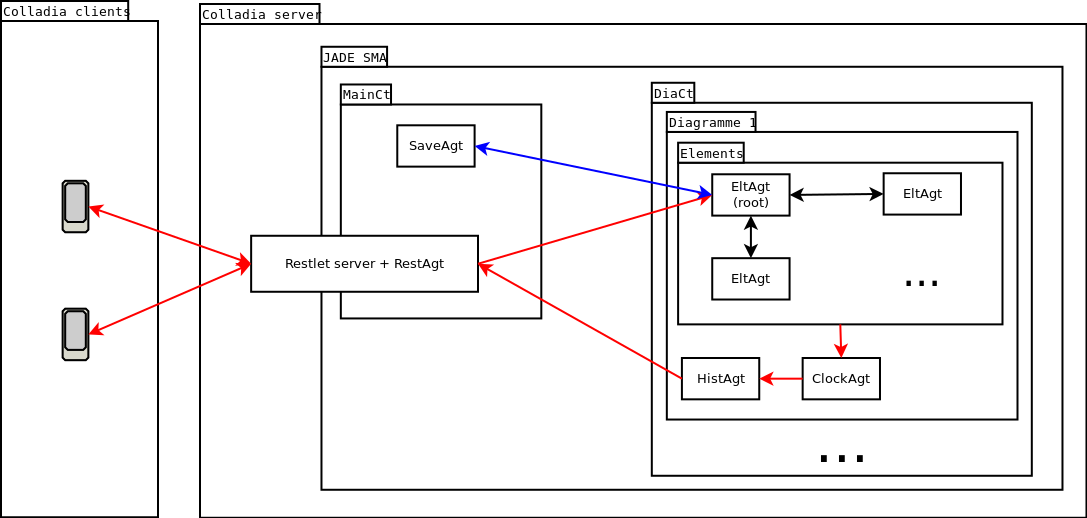
\includegraphics[width=.9\textwidth]{img/general_server}
	\caption{Schéma de l'architecture générale du serveur}
	\vspace*{-.5cm}
	\end{center}
\end{figure}

\subsection{Description de l'interface REST}
\subsubsection{Champs communs}
Un certain nombre de champs sont communs aux différentes requêtes REST.
Pour les entrées le champ \lstinline$last-clock$, optionnel, permettant au serveur de connaître la dernière valeur de l'horloge logique reçue par le client effectuant la requête.

Pour les sorties, il faut commencer par différencier les modifications sauvegardées par l'agent historique du message de retour des requêtes REST.
Le retour comporte obligatoirement un champ \lstinline$status$ contenant un code d'erreur et un champ \lstinline$clock$ donnant la dernière valeur de l'horloge logique du diagramme.
Le champ \lstinline$status$ peut prendre une des valeurs suivantes, inspirées des standards web :
\begin{itemize}
	\item succès (2xx) :
	\begin{itemize}
		\item 200 : OK
	\end{itemize}
	\item redirection (3xx) :
	\begin{itemize}
		\item 304 : non-modifié
	\end{itemize}
	\item erreur client (4xx) :
	\begin{itemize}
		\item 400 : requête mal formée
		\item 401 : existe déjà
		\item 404 : non-trouvé
	\end{itemize}
	\item erreur serveur (5xx) :
	\begin{itemize}
		\item 500 : erreur interne
	\end{itemize}
\end{itemize}
Dans le cas où la requête n'a pas pu être exécutée (\lstinline$status != 200$), un champ \lstinline$error$ est intégré au retour contenant une description de l'erreur.
Si la requête à été exécutée correctement, qu'un champ \lstinline$last-clock$ a été spécifiée par le client et que sa valeur est valide par rapport aux modifications enregistrées par l'HistAgt du diagramme, alors on renvoie un champ \lstinline$modification-list$ qui est un tableau JSON contenant un ensemble de modifications telles que décrites ci-après.
Si on est dans l'incapacité de produire une liste de modifications, on retourne un champ \lstinline$description$ contenant une description complète du diagramme et de ses sous-éléments sous-forme d'une sérialisation JSON.

Les modifications engendrées par certains types de requêtes (PUT, POST et DELETE) et stockées dans l'agent d'historique comportent forcément un champ \lstinline$clock$ indiquant l'horloge à laquelle la modification a eu lieu et un champ \lstinline$type$ donnant le type de la modification (PUT, POST ou DELETE).

\subsubsection{Requêtes GET}
Les requêtes de type GET permettent d'obtenir des informations sur l'état actuel du diagramme et n'engendrent jamais de modifications.
Si l'URI est de la forme \lstinline$<server adress>$, renvoie un champ \lstinline$list$ contenant un tableau JSON des noms des différents diagrammes stockés sur le serveur.

Si l'URI est de la forme \lstinline$<server adress>/<diagram>[/<element> ...]$, renvoie un champ \lstinline$path$ donnant le chemin vers l'élément ciblé sous forme d'un tableau JSON ainsi qu'un champ \lstinline$description$ contenant la description récursive de cet élément.

\subsubsection{Requêtes PUT}
Les requêtes de type PUT permettent de créer de nouveaux diagrammes ou de nouveaux sous-éléments.
Si l'URI est de la forme \lstinline$<server adress>/<diagram>$ c'est une création de diagramme, et dans le cas d'un succès (un diagramme possédant le même nom n'existe pas encore), on renvoie un champ \lstinline$path$ contenant le nom du diagramme.

Si l'URI cible un élément (\lstinline$<server adress>/<diagram>/<element[/<element> ...]>$), on créé un nouveau sous-élément.
La requête peut optionnellement contenir un champ \lstinline$properties$ contenant des couples (propriété, valeur) pour initialiser les propriétés de l’élément.
Le retour contient un champ \lstinline$path$ ainsi qu'un champ \lstinline$properties$ contenant une description des propriétés de l'élément venant d'être créé.

\subsubsection{Requêtes DELETE}
Les requêtes de type DELETE permettent de supprimer un EltAgt ou bien une partie de ses propriétés.
Dans les deux cas, l'URI est de la forme \lstinline$<adrr>/<diagram>[/<element> ...]$.
Si la requête possède un champ \lstinline$properties-list$ contenant une liste de nom de propriété à supprimer, alors on supprime uniquement ces propriétés au niveau de l'élément ciblé.
Sinon, on supprime l'EltAgt ciblé ainsi que tous ses fils récursivement.
Dans les deux cas, la modification a la même forme que la requête initiale, à ceci-près que le chemin de l'URI est intégré dans un champ \lstinline$path$ et le type de la requête dans un champ \lstinline$type$.

\subsubsection{Requêtes POST}
Les requêtes REST de type POST permettent de modifier la valeur des propriétés d'un élément, une option permet d’exécuter un algorithme d'auto-positionnement sur les fils d'un EltAgt ciblé.
Dans les deux cas, l'URI est de la forme \lstinline$<adrr>/<diagram>[/<element> ...]$.
Pour modifier directement des propriétés, un champ \lstinline$properties$ contenant des couples (propriété, valeur) doit être spécifié dans la requête.
La modification possède une forme identique à la requête initiale.

Pour exécuter l'algorithme d'auto-positionnement, il faut spécifier dans la requête un champ \lstinline$options$ associé à une liste JSON contenant une valeur \lstinline$auto-positioning$.
Cette requête induit la sauvegarde de 0+ modifications de type POST, une par fils auto-positionnable. Un fils est dit auto-positionnable si il contient des propriétés suffisantes pour permettre un repositionnement, dans notre cas \lstinline$xMin$, \lstinline$xMax$, \lstinline$yMin$ et \lstinline$yMax$.
Chaque modification enregistrée contient un champ \lstinline$path$ contenant le chemin de l'EltAgt modifié ainsi qu'un champ \lstinline$properties$ récapitulant les altérations effectuées.

\newpage
\subsection{Description des agents et des comportements}
\subsubsection{RestAgt}
Le RestAgt est couplé à une classe définissant un serveur Restlet de manière à pouvoir récupérer des requêtes REST puis à les transférer aux agents pouvant y répondre.
L'agent est aussi responsable de la création des nouveaux diagrammes (PUT) et de fournir aux clients la liste des diagrammes existant sur le serveur (GET).
À sa création, le RestAgt s'enregistre auprès du Directory Facilitator (DF) en tant qu'interface REST.

On peut dénombrer deux comportements pour cet agent.
Le premier n'est pas une classe fille de la classe Behaviour, mais on peut considérer que le fait d'attendre les requêtes REST au niveau du serveur Restlet rentre dans la catégorie du comportement au sens multi-agent du terme.
À la réception d'une requête, créé un nouveau diagramme ou retourne la liste des diagrammes disponibles si besoin.
Sinon, envoie la requête sous forme de message ACL au EltAgt racine du diagramme ciblé par la requête et lance un ReceiveBhv.
L'AID du ClockAgt du diagramme est aussi insérée au niveau du champ \lstinline$reply-to$ du message.
Le \lstinline$conversation-id$ est généré par la classe Java UUID.

Le ReceiveBhv attend un message de retour pour une requête envoyée précédemment puis formule la réponse à la requête REST initiale du client.

\subsubsection{SaveAgt}
Le SaveAgt est responsable de la sauvegarde et de la restauration de l'état des diagrammes après un éventuel redémarrage du serveur.
La description de chaque diagramme est stocké dans un fichier au format JSON.
Le premier comportement, dit RestoreBhv, est un OneShotBehaviour lancé au démarrage de l'agent et qui, à partir des données sauvegardées, créé les différents diagrammes (EltAgt racine + ClockAgt + HistAgt) et envoie un message au nouveau EltAgt pour restaurer la valeur de ses propriétés et de ses sous-éléments.
Une fois les différents messages envoyés, lance le TickerBhv et le ReceiveBhv.

Le TickerBhv est un comportement chargé d'envoyer régulièrement des messages GET aux différents EltAgt racine des diagrammes pour récupérer leur description complète.
Le ReceiveBhv est un comportement cyclique qui récupère les réponses à ces messages et écrit les descriptions reçues dans des fichiers .json.

\subsubsection{ClockAgt}
Le ClockAgt est chargé de gérer l'horloge du diagramme et exprime un unique comportement cyclique, le ReceiveBhv.
Il attend un message de type INFORM provenant d'un EltAgt, incrémente l'horloge si le message ne comporte par d'option \lstinline$no-history$ et est de type POST, PUT ou DELETE, puis, dans tous les cas, ajoute un champ \lstinline$clock$ au message comportant la valeur la plus récente de l'horloge.
Le message est ensuite envoyé au HistAgt.

\subsubsection{HistAgt}
Le HistAgt est l'agent chargé de gérer l'historique des modifications et comporte un unique CyclicBehaviour encore une fois nommé ReceiveBhv.
Il réceptionne les messages envoyés par le ClockAgt, et si le message ne comporte par d'option \lstinline$no-history$ et est de type POST, PUT ou DELETE, ajoute le contenu du message, la modification, à l'historique.

L'HistAgt est aussi chargé de formuler la réponse à la requête REST initiale si le message reçu du ClockAgt ne comporte pas une option \lstinline$no-reply$.
Dans ce cas, si le message intègre un champ \lstinline$last-clock$ et que sa valeur est supérieure à l'horloge de la première modification encore stockée dans la liste des modifications, l'agent renvoie au RestAgt la liste des modifications appliquée depuis celle portant l'horloge \lstinline$last-clock$.
Sinon envoie un message au EltAgt racine pour récupérer la description complète du diagramme en ajoutant un champ \lstinline$reply-to$ vers le RestAgt.

\subsubsection{EltAgt}
Agent chargé de stocker l'état courant d'un élément ou du diagramme lui-même.
Pour chaque diagramme, les EltAgt forment une arborescence et la racine, qui représente le diagramme en soi, s'enregistre auprès du DF.
Chaque EltAgt implémente des fonctions permettant entre autre d'ajouter, supprimer, modifier des éléments.
C'est aussi eux qui délibèrent pour permettre un auto-positionnement des éléments à la demande du client.

\paragraph{ReceiveBhv}
Le principal comportement utilisé, le ReceiveBhv, est un CyclicBehaviour lancé au démarrage de l'agent et qui attend des messages de requêtes des autres agents, que ce soit du RestAgt, du SaveAgt ou d'un autre EltAgt du diagramme.
Le fonctionnement de ce comportement après réception d'un message de type REQUEST peut être résumé comme ceci :
\begin{itemize}
	\item PUT :
	\begin{itemize}
		\item Si l'élément courant est l'avant-dernier élément de l'URI, ajoute un nouvel élément si celui-ci n'existe pas déjà (création d'un EltAgt et ajout à l'arborescence).
		\item Sinon, transfert du message au fils correspondant au prochain élément dans l'URI si il existe ou retourne une erreur.
	\end{itemize}
  \item GET :
	\begin{itemize}
		\item Si l'élément courant a une profondeur dans l'arborescence strictement inférieure à celle de la cible de l'URI, transfert du message au fils correspondant au prochain élément dans l'URI si il existe ou retourne une erreur.
		\item Sinon :
		\begin{itemize}
			\item Si l'élément est une feuille, répond au message en envoyant la liste des propriétés et leurs valeurs.
			\item Sinon, transfert le message à tous les sous-éléments et lance un comportement WaitDescriptionBhv pour attendre les réponses.
		\end{itemize}
	\end{itemize}
	\newpage
	\item DELETE :
	\begin{itemize}
		\item Si la requête contient un champ \lstinline$properties-list$ (suppression de propriété) :
		\begin{itemize}
			\item Si l'élément courant est le dernier élément de l'URI, suppression des propriétés dans l'élément si elles existent.
			\item Sinon, transfert du message au fils correspondant au prochain élément dans l'URI si il existe ou retourne une erreur.
		\end{itemize}
		\item Sinon (suppression d'élément) :
		\begin{itemize}
			\item Si l'élément courant a une profondeur dans l'arborescence strictement inférieure à celle de la cible de l'URI, transfert du message au fils correspondant au prochain élément dans l'URI si il existe ou retourne une erreur.
			\item Sinon :
			\begin{itemize}
				\item Si l'élément courant est le dernier élément de l'URI, envoie une réponse à l'expéditeur initiale de la requête.
				\item Transfert du message à tous les fils.
				\item Autodestruction de l'agent.
			\end{itemize}
		\end{itemize}
	\end{itemize}
	\item POST :
	\begin{itemize}
		\item Si l'élément courant est le dernier élément de l'URI :
		\begin{itemize}
			\item Si le message comporte une option \lstinline$auto-positioning$ (auto-positionnement des fils) :
			\begin{itemize}
				\item Envoi un message de type CFP (Call For Proposal) à tous les fils comportant un angle pour la dispersion ainsi que la largeur et la longueur de l'élément courant pouvant prendre la valeur -1 pour indiquer une taille infinie.
				\item Lance un nouveau comportement WaitProposalBhv avec en paramètre le nombre de messages envoyés vers les fils.
			\end{itemize}
			\item Sinon, si le message comporte un champ \lstinline$properties$, modification des propriétés de l'élément et envoi une réponse à l'expéditeur initial de la requête.
		\end{itemize}
		\item Sinon, transfert du message au fils correspondant au prochain élément dans l'URI si il existe ou retourne une erreur.
	\end{itemize}
	\item RESTORE (type supplémentaire du serveur pour la restauration des diagrammes) :
	\begin{itemize}
		\item Pour chaque couple (clef, valeur) du champ \lstinline$properties$ :
		\begin{itemize}
			\item Si la valeur est un objet JSON, créé un nouvel élément, l'ajoute à l'arborescence et lui envoie un message de restauration contenant la valeur du couple.
			\item Sinon, c'est une propriété, et on l'ajoute à celles de l'élément courant.
		\end{itemize}
	\end{itemize}
\end{itemize}

\newpage
\paragraph{Autres comportements}
Le comportement WaitDescriptionBhv est lancé après avoir envoyé des messages aux fils suite à un GET et attend leurs descriptions respectives.
Une fois la description de tous les fils reçus, formule une réponse au message de requête reçu initialement (en prenant en compte le \lstinline$reply-to$).

Le ReceiveCFPBhv est un comportement cyclique lancé au démarrage de l'agent qui, à chaque réception d'un message CFP par l'agent lance un nouveau ProposeBhv.
Ce dernier commence par placer l'élément au centre de son père, puis envoi ses nouvelles coordonnées (\lstinline$x$ et \lstinline$y$) ainsi que ses dimensions (\lstinline$width$ et \lstinline$height$) au père dans un message PROPOSE.
Tant que ce dernier renvoi des REJECT\_PROPOSAL, avance d'un pas fixé dans la direction donnée par l'élément père au lancement de l'algorithme d'auto-positionnement.

Une fois un ACCEPT\_PROPOSAL reçu, il envoi un message au HistAgt du diagramme pour enregistrer la modification des coordonnées.
Sachant que plusieurs modifications peuvent être engendrées par une seule requête d'auto-positionnement et qu'une requête REST n'accepte qu'une unique réponse, on ajoute un flag \lstinline$no-reply$ au message, de manière à ce que ce message n'engendre pas une réponse au RestAgt qui serait ensuite transférée au client.

Si, lors d'une itération l'élément ne peut plus se déplacer en x et en y car il a atteint les limites de son père, alors il intègre une option \lstinline$force$ à son message pour forcer l'acceptation de la proposition.
Si l'élément ne comporte pas les propriétés nécessaires aux calculs d'auto-positionnement (\lstinline$xMin$, \lstinline$xMax$, \lstinline$yMin$ et \lstinline$yMax$), il renvoie un message ayant un performatif REFUSE.

Le comportement WaitProposalBhv est lancé au début de chaque algorithme d'auto-positionnement en sachant combien de CFP ont été envoyés à des fils et entretien une liste des coordonnées et dimensions des éléments fils dont la nouvelle position a déjà été acceptée.
À la réception d'un message de type REFUSE, décrémente le compteur de message attendu.
À la réception d'un message PROPOSE, si la nouvelle position de l'élément fils chevauche celle d'un des éléments déjà accepté, retourne un message de type REJECT\_PROPOSAL, sinon, un ACCEPT\_PROPOSAL.

Dans le cas où le message reçu comporte une option \lstinline$force$, renvoie toujours un ACCEPT\_PROPOSAL.
Chaque envoi d'un ACCEPT\_PROPOSAL induit une décrémentation du compteur.
Une fois que le compteur atteint 0, répond au message de requête initial en ajoutant une option \lstinline$no-history$, de manière à fournir une réponse à la requête REST incluant uniquement les modifications réalisées par ses fils.

\newpage
\subsection{Description des messages}
Pour tous les types de message décrits ci-après, le champ \lstinline$conversation-id$ est un UUID unique généré lors de la réception d'une requête REST par le serveur Restlet.
Tous les messages ACL généré suite à cette requête utilisent ce même identifiant.
Le champ FIPA \lstinline$content$ est toujours un dictionnaire JSON sérialisé.
Les champs utilisés ci-dessous ne faisant pas parti du formalisme FIPA sont des champs de ce dictionnaire.

\subsubsection{RestAgt}
Tous les messages envoyés par le RestAgt respectent le patron suivant :
\begin{itemize}
	\item \lstinline$performative$ : REQUEST
	\item \lstinline$receivers$ : un EltAgt racine
	\item \lstinline$reply-to$ : ClockAgt
	\item \lstinline$type$ : PUT, GET, DELETE ou POST dépendant du type de la requête REST initiale
	\item \lstinline$path$ : chemin du diagramme élément visé par la requête sous forme de tableau JSON
	\item \lstinline$properties$ : liste des propriétés et de leurs valeurs dans le cas d'une modification/création d'un élément
	\item \lstinline$properties-list$ : liste des propriétés à supprimer au sein d'un élément pour certaines requêtes DELETE
	\item \lstinline$options$ : \lstinline$[auto-positionning]$
	\item \lstinline$last-clock$ : dernière horloge reçue par le client si spécifiée dans la requête REST
\end{itemize}

\subsubsection{SaveAgt}
Au démarrage du serveur, envoi des messages respectant le format suivant aux nouveaux EltAgt créés de manière à restaurer l'état du diagramme :
\begin{itemize}
	\item \lstinline$performative$ : REQUEST
	\item \lstinline$receivers$ : un EltAgt racine (une fois créé)
	\item \lstinline$type$ : RESTORE
	\item \lstinline$description$ : description récursive des propriétés du diagramme et de ses éléments sous forme de dictionnaires JSON imbriqués
\end{itemize}
~\\
Une fois la phase de restauration terminée, le SaveAgt envoi à chaque tick de son TickerBhv le message suivant à tous les EltAgt racine :
\begin{itemize}
	\item \lstinline$performative$ : REQUEST
	\item \lstinline$receivers$ : tous les EltAgt racine
	\item \lstinline$type$ : GET
	\item \lstinline$path$ : \lstinline$[]$ (liste vide pour que l'EltAgt retourne la description complète du diagramme)
\end{itemize}

\subsubsection{ClockAgt}
Les messages reçus par le ClockAgt sont transférés au HistAgt après ajout d'un champ \lstinline$clock$, et respectent le format suivant :
\begin{itemize}
	\item \lstinline$performative$ : INFORM
	\item \lstinline$receivers$ : HistAgt
	\item \lstinline$content$ : identique à celui du message reçu avec ajout d'un champ \lstinline$clock$ contenant la dernière valeur de l'horloge logique du diagramme
\end{itemize}

\subsubsection{HistAgt}
Si le HistAgt a pu récupérer la liste des modifications demandées par le client, envoi le message suivant au RestAgt :
\begin{itemize}
	\item \lstinline$performative$ : INFORM
	\item \lstinline$receivers$ : RestAgt
	\item \lstinline$status$ : 200
	\item \lstinline$clock$ : dernière valeur de l'horloge logique (récupérée à partir du dernier message reçu)
	\item \lstinline$modification-list$ : liste des modifications appliquées au diagramme depuis l'horloge \lstinline$last-clock$ spécifiée par le client
\end{itemize}
~\\
Sinon, on envoie un message au EltAgt racine pour obtenir la description complète du diagramme et la transférer au RestAgt :
\begin{itemize}
	\item \lstinline$performative$ : INFORM
	\item \lstinline$receivers$ : EltAgt racine
	\item \lstinline$reply-to$ : RestAgt
	\item \lstinline$type$ : GET
	\item \lstinline$path$ : \lstinline$[]$ (liste vide pour que l'EltAgt retourne la description complète du diagramme)
	\item \lstinline$clock$ : valeur de l'horloge logique insérée dans le contenu du message par le ClockAgt
\end{itemize}

\subsubsection{EltAgt}
Au niveau des éléments, on peut distinguer deux grandes familles de messages, les messages internes, envoyés d'un EltAgt à un autre EltAgt de l'arborescence, et les messages qui ont pour destinataires d'autres agents du diagramme (ClockAgt, RestAgt, etc.).
Pour les messages dirigés vers l'extérieur, il existe deux possibilités.
Soit l’exécution de la requête s'est déroulée sans encombres :
\begin{itemize}
	\item \lstinline$performative$ : INFORM
	\item \lstinline$receivers$ : valeur du champ \lstinline$reply-to$, ou \lstinline$sender$ si le premier est inexistant	
  \item \lstinline$status$ : 200
  \item \lstinline$content$ : contenu de la requête initial plus les éventuels champs suivants :
  \item \lstinline$description$ : description récursive d'un élément du diagramme ou du diagramme complet dans le cas d'une requête GET
\end{itemize}

Soit elle a générée une erreur :
\begin{itemize}
	\item \lstinline$performative$ : FAILURE
	\item \lstinline$receivers$ : valeur du champ \lstinline$sender$ de la requête (le \lstinline$reply-to$ est ignoré)
  \item \lstinline$status$ : un code d'erreur (3xx, 4xx ou 5xx)
  \item \lstinline$error$ : message de description de l'erreur
\end{itemize}
~\\
Pour les messages internes, on peut distinguer deux types de messages en plus de ceux liés à l'algorithme d'auto-positionnement.
Lors du transfert d'un message vers le prochain fils de l'URI, l’entièreté des champs du message sont conservés, \lstinline$reply-to$ et \lstinline$sender$ compris.

Pour ce qui est des requêtes GET en revanche, une fois que la cible de l'URI a été passée, les messages envoyés aux différents fils en supprimant le champ \lstinline$reply-to$ et en mettant l'AID de l'EltAgt courant dans le champ \lstinline$sender$.
Ainsi, une fois qu'un élément à récupéré récursivement sa description, il crée une réponse au message de requête reçu.
Le destinataire sera alors l'agent externe à l'arborescence ayant envoyé la requête ou le \lstinline$reply-to$ qu'il a spécifié si l'agent courant était la cible de l'URI, ou bien le père dans l'arborescence des éléments du diagramme.

\paragraph{Messages liés à l'algorithme d'auto-positionnement}
À la réception d'une demande d'auto-positionnement, la cible de l'URI transfère à tous ces fils un message respectant le format suivant :
\begin{itemize}
	\item \lstinline$performative$ : CFP
	\item \lstinline$receivers$ : un EltAgt fils
	\item \lstinline$x$, \lstinline$y$, \lstinline$width$ et \lstinline$height$ : valeurs calculées à partir des propriétés \lstinline$xMin$, \lstinline$xMax$, \lstinline$yMin$ et \lstinline$yMax$ de l'élément
	\item \lstinline$angle$ : un angle de dérivation donné par la formule $\frac{2 \pi}{n} * i$ où $n$ est le nombre de fils et $i$ l'index du fils dans la liste des fils
\end{itemize}
~\\
L'EltAgt recevant ce message renvoi alors un message REFUSE si il n'est pas auto-positionnable :
\begin{itemize}
	\item \lstinline$performative$ : REFUSE
	\item \lstinline$receivers$ : EltAgt père dont l'AID est donnée par le champ \lstinline$sender$ du CFP reçu
\end{itemize}
~\\
Une proposition dans le cas contraire ou si un REJECT\_PROPOSAL a été reçu de la part du père suite à une proposition :
\begin{itemize}
	\item \lstinline$performative$ : PROPOSE
	\item \lstinline$receivers$ : EltAgt père dont l'AID est donnée par le champ \lstinline$sender$ du dernier message CFP ou REJECT\_PROPOSAL reçu
	\item \lstinline$x$, \lstinline$y$, \lstinline$width$ et \lstinline$height$ : nouvelles coordonnées proposées ainsi que les dimensions pour vérifier l'existence de chevauchement
	\item \lstinline$options$ : \lstinline$[force]$ si l'élément a atteint les limites de son père
\end{itemize}
~\\
Les messages permettant d'accepter ou de refuser une proposition sont relativement simples :
\begin{itemize}
	\item \lstinline$performative$ : REJECT\_PROPOSAL ou ACCEPT\_PROPOSAL
	\item \lstinline$receivers$ : L'EltAgt fils ayant soumis une proposition
\end{itemize}

Une fois qu'un élément a vu sa proposition acceptée, il envoie un message contenant ses nouvelles coordonnées pour le HistAgt :
\begin{itemize}
	\item \lstinline$perfomative$ : INFORM
	\item \lstinline$receivers$ : ClockAgt
	\item \lstinline$type$ : POST
	\item \lstinline$properties$ : \lstinline${xMin:<value>, xMax:<value>, yMin:<value>, yMax:<value>}$
	\item \lstinline$options$ : \lstinline$[no-reply, auto-positionning]$
\end{itemize}
~\\
Une fois l'auto-positionnement de tous les fils réalisés, l'EltAgt père envoi un message au HistAgt pour qu'une réponse soit formulée à la requête REST initiale :
\begin{itemize}
	\item \lstinline$perfomative$ : INFORM
	\item \lstinline$receivers$ : ClockAgt
	\item \lstinline$options$ : \lstinline$[no-history, auto-positionning]$
\end{itemize}

\subsection{Limites et améliorations}
Concernant la partie serveur du projet on peut noter quelques points qui serait potentiellement limitants dans le cadre d'un déploiement à grande échelle :
\begin{itemize}
	\item
	À part pour l'auto-positionnement, le serveur manipule les données envoyées par les clients sans se préoccuper de leur nature.
	Pour ce faire, toutes les données sont stockées sous forme de string et ce récursivement.
	Le contenu des messages transitant à la fois entre les différents agents et entre les clients et le serveur comporte de ce fait un grand nombre de caractères '\textbackslash' utilisés pour échapper les caractères de début de chaîne ('"').
	Pour des arborescences ayant une certaine profondeur, ceci pourrait être défavorable car les messages pourraient finir par contenir plus de caractères d'échappement que de caractères utiles.
	\item
	Le fait d'utiliser la technologie REST implique que les clients doivent réaliser régulièrement (un centième de seconde au moment de l'écriture de ce rapport) des requêtes de type GET pour être tenus informés des modifications produites par les autres clients.
	Si beaucoup de clients étaient connectés simultanément à un même serveur, celui-ci pourrait en pâtir.
	Pour éviter ce problème, il faudrait faire le choix d'une autre technologie bidirectionnelle, tel que les sockets.
\end{itemize}

L'algorithme d'auto-positionnement pourrait quant à lui aussi être amélioré sur certains points :
\begin{itemize}
	\item Prise en compte des liens pour le positionnement.
	\item Redimensionnement intelligent des fils en fonction de leur contenu.
	\item Ajustement de la taille de police des textes.
\end{itemize}


\section{Conclusion}
Au cours de ce projet, il nous a été possible d'utiliser à la fois les notions du cours de IA04 et de NF28 ce qui nous a permis d'approfondir nos connaissances dans ces domaines.
De plus, le fait de travailler à 5 sur ce projet nous a demandé de communiquer et d'organiser la répartition des tâches de manière continue sur toute la durée du projet. Il a ainsi fallu utiliser des outils tel que Slack pour communiquer, git pour gérer les versions du code et Google Drive pour partager des documents.
Les difficultés rencontrés nous ont amenés à échanger nos idées pour permettre de les résoudre de la manière la plus adapté possible, en se servant de l'expérience de chacun. 
Cela a été un réel plaisir d'avoir travailler sur ce projet et nous avons pu apprendre beaucoup que se soit au nouveau de la conception, ou de la programmation Android.


\end{document}
